\documentclass{article}

\usepackage{indentfirst}
\usepackage{amssymb,amsmath,mathtools,bm,mathabx}
\usepackage{graphicx}
\usepackage{calc}
\usepackage{rotating}
\usepackage{multirow}
\usepackage{eurosym}
\usepackage{wrapfig}
\usepackage{mathdots}
\usepackage[a4paper,margin=0.3mm,paperwidth=20.9cm,paperheight=29.5cm]{geometry}
\usepackage{tikz,tikzsymbols}
\usetikzlibrary{calc}
\usepackage{color,soul}
\usepackage{float}
\usepackage{parskip}
\usepackage{colortbl}
\usepackage{stackengine}
\usepackage{scalerel}
\usepackage{tcolorbox}
\usepackage{multicol}
\usepackage{tabularx}
\usepackage[inline]{enumitem}
\usepackage[framemethod=tikz]{mdframed}
\usepackage{adjustbox}
\usepackage{sidecap}
\usepackage{enumitem}
%\usepackage{newclude}
\usepackage{hyperref}
\hypersetup{
    % Something here
    colorlinks=true,
    linkcolor=blue
}
\usepackage{algorithm}
\usepackage{algpseudocode}

\hfuzz=400pt
\vfuzz=400pt

\setlist{nosep}

\setlength{\columnseprule}{0.4pt}
\setlength{\columnsep}{0pt}

\makeatletter
\g@addto@macro\normalsize{%
  \setlength\abovedisplayskip{0pt}
  \setlength\belowdisplayskip{0pt}
  \setlength\abovedisplayshortskip{0pt}
  \setlength\belowdisplayshortskip{0pt}
}
\makeatother

\makeatletter
\renewcommand*\env@matrix[1][*\c@MaxMatrixCols c]{%
  \hskip -\arraycolsep
  \let\@ifnextchar\new@ifnextchar
  \array{#1}}
\makeatother

\definecolor{mycolor}{rgb}{0.122, 0.435, 0.698}

\setlength{\parindent}{0pt}
\setlength{\parskip}{0pt}
\renewcommand{\baselinestretch}{1}

% \usepackage{tikzpagenodes}
% \usepackage{background}
% \backgroundsetup%
% {   contents={
%         \begin{tikzpicture}[overlay]
%             \draw[black!100] ($(current page text area.south west)+(-0.05,-0.05)$) rectangle ($(current page text area.north east)+(0.05,0.05)$);
%         \end{tikzpicture}
%     },
%     scale=1,
%     angle=0,
%     opacity=1
% }
\newlength{\boxskiplength}
\newlength{\innermarginlength}
\setlength{\boxskiplength}{0pt}
\setlength{\innermarginlength}{1.4pt}

\newmdenv[
skipabove=\boxskiplength,
backgroundcolor=orange!90,
innerleftmargin=\innermarginlength,
innerrightmargin=\innermarginlength,
innertopmargin=\innermarginlength,
innerbottommargin=\innermarginlength,
middlelinewidth=0pt
]
{Chapter}

\newmdenv[
skipabove=\boxskiplength,
backgroundcolor=yellow!50,
innerleftmargin=\innermarginlength,
innerrightmargin=\innermarginlength,
innertopmargin=\innermarginlength,
innerbottommargin=\innermarginlength,
middlelinewidth=0pt
]
{Subchapter}

\newmdenv[
skipabove=\boxskiplength,
backgroundcolor=green!40,
innerleftmargin=\innermarginlength,
innerrightmargin=\innermarginlength,
innertopmargin=\innermarginlength,
innerbottommargin=\innermarginlength,
middlelinewidth=0pt
]
{Definition}

\newmdenv[
skipabove=\boxskiplength,
backgroundcolor=red!40,
innerleftmargin=\innermarginlength,
innerrightmargin=\innermarginlength,
innertopmargin=\innermarginlength,
innerbottommargin=\innermarginlength,
middlelinewidth=0pt
]
{Theorem}

\newmdenv[
skipabove=\boxskiplength,
backgroundcolor=blue!40,
innerleftmargin=\innermarginlength,
innerrightmargin=\innermarginlength,
innertopmargin=\innermarginlength,
innerbottommargin=\innermarginlength,
middlelinewidth=0pt
]
{Fact}

\newmdenv[
skipabove=\boxskiplength,
backgroundcolor=orange!40,
innerleftmargin=\innermarginlength,
innerrightmargin=\innermarginlength,
innertopmargin=\innermarginlength,
innerbottommargin=\innermarginlength,
middlelinewidth=0pt
]
{Corollary}

\newmdenv[
skipabove=\boxskiplength,
backgroundcolor=black!40,
innerleftmargin=\innermarginlength,
innerrightmargin=\innermarginlength,
innertopmargin=\innermarginlength,
innerbottommargin=\innermarginlength,
middlelinewidth=0pt
]
{Proof}

\newmdenv[
skipabove=\boxskiplength,
backgroundcolor=cyan!40,
innerleftmargin=\innermarginlength,
innerrightmargin=\innermarginlength,
innertopmargin=\innermarginlength,
innerbottommargin=\innermarginlength,
middlelinewidth=0pt
]
{Example}

\newmdenv[
skipabove=\boxskiplength,
backgroundcolor=magenta!40,
innerleftmargin=\innermarginlength,
innerrightmargin=\innermarginlength,
innertopmargin=\innermarginlength,
innerbottommargin=\innermarginlength,
middlelinewidth=0pt
]
{Method}

\newmdenv[
skipabove=\boxskiplength,
backgroundcolor=yellow!40,
innerleftmargin=\innermarginlength,
innerrightmargin=\innermarginlength,
innertopmargin=\innermarginlength,
innerbottommargin=\innermarginlength,
middlelinewidth=0pt
]
{InnerMethod}
\newcommand*{\QED}{\ensuremath{\blacksquare}}
\newcommand{\union}{\cup}
\newcommand{\intersection}{\cap}
\newcommand{\overeq}[1]{\stackrel{\mathclap{\tiny{\substack{#1}}}}{=}}
\newcommand{\overto}[1]{\stackrel{\mathclap{\tiny{\substack{#1}}}}{\to}}
\newcommand{\Adj}{\textsc{Adj}}
\newcommand{\linA}{\mathcal{A}}
\newcommand{\linB}{\mathcal{B}}
\newcommand{\linC}{\mathcal{C}}
\newcommand{\inv}{^{-1}}
\newcommand{\perpoplus}{\overset{\perp}{\oplus}}
\newcommand{\e}[1]{e^{#1}}
\newcommand{\inver}[1]{#1^{-1}}
\newcommand{\fnorm}[2]{\|#1\|_{#2}}
\newcommand{\Property}[1]{
	\begin{properties}
		\item[\textit{Property #1}.]
	\end{properties}
}
\newcommand{\skewmat}[1]{\bm{#1}^{\times}}
\newcommand{\proj}[2]{\text{proj}_{#1}(#2)}
\newcommand{\tabitem}{~~\llap{\textbullet}~~}
\newcommand{\basis}[3]{\{#1_{#2}\}_{#2=1}^{#3}}
\newcommand{\sequence}[3]{\{#1_{#2}\}_{#2=0}^{#3}}
\newcommand{\Naturals}{\mathbb N}
\newcommand{\Reals}{\mathbb R}
\newcommand{\Complex}{\mathbb C}
\newcommand{\argmin}{\operatornamewithlimits{argmin}}
\newcommand{\argmax}{\operatornamewithlimits{argmax}}
\newcommand{\then}{\Rightarrow}
\newcommand{\Rank}{\textsc{Rank}}
\newcommand{\Range}{\textsc{Range}}
\newcommand{\Nullity}{\textsc{Nullity}}
\newcommand{\Null}{\textsc{Null}}
\newcommand{\Det}{\textsc{Det}}
\newcommand{\Spec}{\textsc{Spec}}
\newcommand{\DIM}{\text{dim}}
\newcommand*\bigcdot{\mathpalette\bigcdot@{.5}}
\newcommand{\InnerProd}[2]{\langle#1,#2\rangle}
\newcommand{\scaleval}{0.8}
\newcommand{\Expectation}[1]{\mathbb{E}\left[#1\right]}
\newcommand{\Variance}[1]{\text{Var}[#1]}
\newcommand{\Cov}[2]{\text{Cov}[#1,#2]}
\newcommand{\Prob}{\mathbb P}
\newcommand{\ord}[1]{^{\left(#1\right)}}
\DeclarePairedDelimiter\ceil{\lceil}{\rceil}
\DeclarePairedDelimiter\floor{\lfloor}{\rfloor}
\newcommand{\mc}[2]{{\color{#1}#2}}

%%%%%%%%%% Drawings
\newcommand*\circled[1]{\tikz[baseline=(char.base)]{\node[shape=circle,draw,inner sep=0pt,minimum size=0.1em] (char) {#1};}}

\newcommand*\circledcolor[2]{\tikz[baseline=(char.base)]{\node[shape=circle,draw,inner sep=0pt,minimum size=0em,fill=#2] (char) {#1};}}

\newcommand*\squaredcolor[2]{\tikz[baseline=(char.base)]{\node[shape=rectangle,draw,inner sep=0.5pt,minimum size=0.1em,fill=#2] (char) {#1};}}

\newcommand*\squaredcolornobord[2]{\tikz[baseline=(char.base)]{\node[shape=rectangle,inner sep=0.5pt,minimum size=0.1em,fill=#2] (char) {#1};}}

\newcommand\dangersign[1][1.5em]{%
  \renewcommand\stacktype{L}%
  \scaleto{\stackon[0.7pt]{\color{red}$\triangle$}{\tiny !}}{#1}%
}

%%%%%%%%%% Big commands
\newcommand{\distribdiscript}[6]{
\noindent\rule[0ex]{\linewidth}{0.5pt}
\flushleft{\textbf{#1 ($X\sim #2$)}} % Name (#1) and notation (#2)
\vspace{-2mm}
\noindent\rule[1.5ex]{\linewidth}{0.5pt}
#3 % Description of distribution
\begin{tabularx}{1\columnwidth}{X|X}
\hline
#4 % PMF/PDF/CDF go here
&
Properties:
#5 % Properties of distribution go here
\\ \hline
\end{tabularx}
\myfigure{
\includegraphics[width=0.9\columnwidth]{#6.pdf} % Filename of the distribution grpahic goes here
}
}

\newcommand{\nextchapter}[1]{
\begin{Chapter}
	\addtocounter{section}{1}
	\textbf{\thesection: #1}
\end{Chapter}
}

\newcommand{\nextsubchapter}[1]{
\begin{Subchapter}
	\textbf{#1}
\end{Subchapter}
}

\newcommand{\myfigure}[1]{
\vspace{-4mm}
\begin{figure}[H]
\centering
#1
\end{figure}
\vspace{-4mm}
}
\usetikzlibrary{shapes,arrows}
\usetikzlibrary{positioning}

\tikzstyle{block} = [draw, fill=blue!20, rectangle, 
    minimum height=1pt, minimum width=1pt]
\tikzstyle{sum} = [draw, fill=blue!20, circle, node distance=1cm]
\tikzstyle{input} = [coordinate]
\tikzstyle{output} = [coordinate]
\tikzstyle{pinstyle} = [pin edge={to-,thin,black}]
\tikzstyle{city} = [draw, fill=white!20, circle, node distance=0.5cm,minimum size=1.1em]
\tikzstyle{box} = [draw, fill=white!20, rectangle, 
    minimum height=1pt, minimum width=1pt]

\begin{document}
\begin{multicols*}{3}
\tiny

\nextchapter{Proofs and functions}

\textbf{By sequence $p\then q$.} Establish $p\then p_1\then \ldots\then p_n\then q$.

\textbf{By induction.} Prove $p_0$ true; assume $p_k$ true; deduce $p_{k+1}$ true.

\textbf{By contraposition $p\then q$.} Prove that $\neg q\then \neg p$.

\textbf{By contradiction $p\then q$.} Show that $p\then\neg q$ gives contradiction.

\textbf{If and only if.} Must prove ($\then$) and ($\Leftarrow$).

\textbf{Set equality}. Prove $A\subseteq B$ (e.g. $x\in A\Rightarrow x\in B$) \& $B\subseteq A$.

\begin{Definition}
$f:X\to Y$. $X$ dom, $Y$ codom, $\{y\in Y|\exists x\in X, f(x)=y\}$ range.
\begin{enumerate*}[label=\protect\circled{\arabic*}]
  \item \textbf{Injective} $\Leftrightarrow f(x_1)=f(x_2)\then x_1=x_2$.
  \item \textbf{Surjective} $\Leftrightarrow \forall y\in Y\exists x\in X\text{, }y=f(x)$.
  \item \textbf{Bijective} $\Leftrightarrow$ inj \& surj.
\end{enumerate*}
\end{Definition}

\begin{Definition}
\begin{enumerate*}[label=\protect\circled{\arabic*}]
  \item $g_L:Y\to X$ left inv $\Leftrightarrow g_L\circ f=1_X$.
  \item $g_R:Y\to X$ right inv $f$ $\Leftrightarrow f\circ g_R=1_Y$.
  \item $g:Y\to X$ inv $\Leftrightarrow$ both left and right inv.
\end{enumerate*}
$f$ invertible if $\exists$ inverse of $f$; then inverse is unique and left$\equiv$right.
\end{Definition}

\begin{Theorem}
\begin{enumerate*}[label=\protect\circled{\arabic*}]
  \item $f$ has left inv $\Leftrightarrow$ injective.
  \item $f$ has right inv $\Leftrightarrow$ surjective.
  \item $f$ invertible $\Leftrightarrow$ bijective.
  \item If $f$ invertible, inverse is unique!
\end{enumerate*}
\end{Theorem}

\begin{Fact}
\begin{flushleft}
\textbf{Func. compos.}
\begin{enumerate*}
\item Associative
\item Compos of injections $\Rightarrow$ injection; surj $\Rightarrow$ surj; bij $\Rightarrow$ bij
\item $(f\circ g)^{-1}=(g^{-1}\circ f^{-1})$.
\end{enumerate*}
\end{flushleft}
\end{Fact}
\nextchapter{Introduction to Algebra}

\begin{Definition}
\textbf{Group} $(G,*)$:
\begin{enumerate*}[label=\protect\circled{\arabic*}]
  \item[\circled{0}] $*$ closed
  \item $*$ assoc: $a*(b*c)=(a*b)*c$
  \item $\exists$ iden $e\in G, a*e=e*a=a$
  \item $\exists a^{-1}\in G, a*a^{-1}=a^{-1}*a=e$
  \item[(4.)] \textbf{Abelian}: $*$ commutative: $a*b=b*a$
\end{enumerate*}
\end{Definition}

\begin{Definition}
\textbf{Ring.}
$(R,+,\cdot)$, bin ops $+:R\times R\to R$ (\textbf{closed} addition), $\cdot:R\times R\to R$ (\textbf{closed} multiplic.) s.t. 
\begin{enumerate}[leftmargin=4mm]
  \item Addition satisfies:
  \begin{itemize*}
    \item Assoc: $a+(b+c)=(a+b)+c$.
    \item Commut: $a+b=b+a$
    \item $\exists$ iden $0\in R$, $a+0=a$.
    \item $\exists$ inv: $(-a)\in R$, $a+(-a)=(-a)+a=0$.
  \end{itemize*}
  \item Multiplication satisf:
  \begin{itemize*}
    \item Assoc: $\forall a,b,c\in R, a\cdot(b\cdot c)=(a\cdot b)\cdot c$.
    \item $\exists$ iden $\exists 1\in R,\forall a\in R,1\cdot a=a\cdot 1=a$.
  \end{itemize*}
  \item Multip. distributive wrt add.: $\forall a,b,c\in R,a\cdot(b+c)=a\cdot b+a\cdot c$ and $(b+c)\cdot a=b\cdot a+c\cdot a$.
  \item[(4)] \textbf{Commutative ring} if $\forall a,b\in R, a\cdot b=b\cdot a$
\end{enumerate}
\end{Definition}

\begin{Fact}
$(R,+,\cdot)$ ring:
\begin{enumerate*}
  \item $a\cdot 0=0\cdot a=0$
  \item $(-a)\cdot b=a\cdot(-b)=-(a\cdot b)$
\end{enumerate*}
\end{Fact}
\begin{Definition}
$\Reals[s]\hspace{-1mm}:\sum_{0}^n a_i s^i$;
$\Reals(s):\sum_{0}^m a_i s^i/\sum_{0}^n b_i s^i$;
$\Reals_p(s):\sum_{0}^n a_i s^i/\sum_{0}^n b_i s^i$
\end{Definition}
\begin{Definition}
\textbf{Field} $(F,+,\cdot)$ commut ring \& $\forall a\in F\setminus0, \exists a^{-1}\in F,a\cdot a^{-1}=1$
\end{Definition}
\begin{Definition}
\textbf{\hl{Linear space (LS)}} $(V,F,\oplus,\odot)$: set $V$ of \textbf{vectors}, field $(F,+,\cdot)$ of \textbf{scalars}, w/ bin ops $\oplus:V\times V\to V$ and $\odot:F\times V\to V$ s.t.
\begin{enumerate}[leftmargin=4mm]
  \item $\oplus$ satisfies:
  \begin{itemize*}
    \item Assoc: $x\oplus(y\oplus z)=(x\oplus y)\oplus z$.
    \item Commut: $x\oplus y=y\oplus x$.
    \item $\exists$ iden $\theta\in V$ s.t. $x\oplus\theta=x$.
    \item $\exists$ inverse: $\forall x\in V,\exists(\ominus x)\in V, x\oplus(\ominus x)=\theta$.
  \end{itemize*}
  \item $\odot$ satisfies:
  \begin{itemize*}
    \item Assoc: $a\odot(b\odot x)=(a\cdot b)\odot x$
    \item Mult by iden $1\in F$ leaves elems unchanged: $\forall x\in V,1\odot x=x$.
  \end{itemize*}
  \item $\odot$ distribut. wrt $\oplus$: $\forall a,b\in F,\forall x,y\in V,(a+b)\odot x=(a\odot x)\oplus(b\odot x)$ and $a\odot(x\oplus y)=(a\odot x)\oplus(a\odot y)$.
\end{enumerate}
\end{Definition}
\begin{Fact}
$(V,F,\oplus,\odot)$ LS:
\begin{enumerate*}
  \item $0\odot x=\theta$
  \item $(-a)\odot x=\ominus(a\odot x)=a\odot(\ominus x)$
\end{enumerate*}
\end{Fact}
\begin{Definition}
\textbf{Product space} $(V\times W,F,\oplus,\odot)$ is LS of pairs $(v,w)\in V\times W$ with $(v_1,w_1)\oplus(v_2,w_2)=(v_1\oplus_V v_2,w_1\oplus_W w_2)$ and $a\odot(v,w)=(a\odot_V v,a\odot_W w)$.
\end{Definition}
\textbf{Def}: $C^k([t_0,t_1],\mathbb R^n)$ LS of $k$-times diffbl funcs $f:[t_0,t_1]\to\mathbb R^n$

\begin{Definition}
\textbf{\hl{Linear subspace (LSS)}} $(W\subseteq V,F)$ of $V\Leftrightarrow$ itself LS, i.e. $\theta_V\in W$ and $\forall w_1,w_2\in W,\forall a_1,a_2\in F$, we have $a_1 w_1+a_2 w_2\in W$.
\end{Definition}
$\{(W_i,F)\}_{i=1}^n$ LSS's of $(V,F)$:
\begin{itemize*}
  \item $\bigcap_{i=1}^n (W_i,F)$ always LSS
  \item $\bigcup_{i=1}^n (W_i,F)$ LSS only if $W_i$ embedded ($\exists W_k$ encompassing all)
\end{itemize*}

\begin{Definition}
LSS of $(V,F)$ gen. by $S$: $\textsc{Span}(S)=\left\{ \sum_{i=1}^n{a_iv_i}|a_i\in F, v_i\in S \right\}$.
\end{Definition}
\begin{Definition}
$\{v_i\}_{i=1}^n$ \textbf{\hl{lin indep}} $\Leftrightarrow$ ($\sum_{i=1}^n{a_i v_i}=0\Leftrightarrow a_i=0, \forall i=1,\ldots,n$).
\end{Definition}
\begin{Definition}
Set $S\subseteq V$ is \textbf{\hl{basis}} of $(V,F)$ $\Leftrightarrow$ it is lin. indep. and $\textsc{Span}(S)=V$.
\end{Definition}
\begin{Fact}
All bases have same \# of elements $=\text{dim}(V)$ (\textbf{dimension} of $V$).
\end{Fact}
\begin{Definition}
\textbf{Representation} $\xi=(\xi_1,\xi_2,\ldots,\xi_n)\in F^n$ of $x\in V$ wrt basis $\basis{b}{i}{n}$ such that $x=\sum_{i=1}^n {\xi_i b_i}$, \textbf{unique} wrt a basis!
\end{Definition}
\begin{Definition}
$\linA:U\to V$ \textbf{linear} $\Leftrightarrow\linA(a_1u_1+a_2u_2)=a_1\linA(u_1)+a_2\linA(u_2)$.
\end{Definition}
\begin{Definition}
$\linA:U\to V$ \begin{itemize*} \item \textbf{null space} $\textsc{Null}(\linA)=\{u\in U|\linA(u)=\theta_V\}\subseteq U$
\item \textbf{range space} $\textsc{Range}(\linA)=\{v\in V|\exists u\in U:v=A(u)\}\subseteq V$
\end{itemize*}
\end{Definition}
\begin{Theorem}
$\linA:U\to V$ \textbf{surjectv} $\Leftrightarrow\textsc{Range}(\linA)=V$; \textbf{injectv} $\Leftrightarrow\textsc{Null}(\linA)=\theta_U$
\end{Theorem}
\begin{Definition}
\textbf{Eigenvalue} $\lambda\in F$ of $\linA:V\to V\Leftrightarrow\exists v\in V\text{ s.t. }v\ne\theta_V\wedge A(v)=\lambda\cdot v$. Then $v$ called \textbf{eigenvector} of $\linA$ for the eigenvalue $\lambda$.
\end{Definition}
\begin{Fact}
The set of eigenvectors $\{v\in V|\linA(v)=\lambda v\}$ is a subspace of $V$.
\end{Fact}
\begin{Theorem}
Given field $F$, every matrix $A\in F^{m\times n}$ defines a linear map $\linA:(F^n,F)\to(F^m,F)$ by matrix multiplication.
\end{Theorem}
\begin{Definition}
$\linA(x)=Ax$: $\Rank(A):=\DIM\Range(\linA)$, $\Nullity(A):=\DIM\Null(\linA)$
\end{Definition}
\begin{Theorem}
$A\in F^{n\times m}$: \begin{itemize*}
\item $\Rank(A)+\Nullity(A)=m$
\end{itemize*}
\begin{itemize}[leftmargin=16.9mm]
  \item $0\le\Rank(A)\le\min\{m,n\}$
  \item If $P\in F^{m\times m}$ and $Q\in F^{n\times n}$ invertible, then:
\begin{equation*}
\hspace{-15mm}
\begin{cases}
\Rank(A)=\Rank(AP)=\Rank(QA)=\Rank(QAP) \\
\Nullity(A)=\Nullity(AP)=\Nullity(QA)=\Nullity(QAP)
\end{cases}
\end{equation*}
\end{itemize}
\end{Theorem}
\begin{Theorem}
Let $A\in F^{n\times n}$ matrix rep of $\linA:F^n\to F^n$, $\linA(x)=Ax$. Equiv:
\begin{enumerate*}
  \item $A$ inv
  \item $\linA$ bij
  \item $\linA$ inj
  \item $\linA$ surj
  \item $\Rank(A)=n$
  \item $\Nullity(A)=0$
  \item $A$ cols are lin indep
  \item $A$ rows are lin indep
\end{enumerate*}
\end{Theorem}
\begin{Theorem}
$A\in F^{n\times n}$:
\begin{itemize*}
  \item $\lambda\in\mathbb C$ eigval of $A$
  \item $\Det(\lambda I-A)=0$
  \item $v\in \mathbb C^n\setminus 0, Av=\lambda v$ \textbf{\hl{r eigvec}}
  \item $\eta\in \mathbb C^n\setminus 0, \eta^TA=\lambda\eta^T$ \textbf{\hl{l eigvec}}
\end{itemize*}
\end{Theorem}
\begin{Definition}
\textbf{\hl{Spectrum}} $\Spec[A\in F^{n\times n}]=\{\lambda_1,\ldots,\lambda_n\}$; $A$ inv $\Leftrightarrow\lambda_i\ne 0\forall i$
\end{Definition}
\begin{Theorem}
Any lin. map $\linA:F^n\to F^m$ between 2 finite-dim. spaces can be represented by a \textbf{unique} matrix $A\in F^{m\times n}$ (wrt fixed bases).
\end{Theorem}
Let $\linA:(U,F)\to(V,F),\basis{u}{j}{n}\to\basis{v}{i}{m}$ then:
\vspace{-1mm}
\begin{equation*}
y_j=\linA(u_j)=\sum_{i=1}^m{a_{ij}v_i}
\Rightarrow A:=\begin{bmatrix}
a_{11}&\cdots&a_{1n}\\
\vdots&\ddots&\vdots\\
a_{m1}&\cdots&a_{mn}
\end{bmatrix}\in F^{m\times n}
\end{equation*}
\begin{Fact}
Let $x=\sum_{j=1}^n\xi_ju_j\in U$, rep of $x$ is $\xi=(\xi_1,\ldots,\xi_n)$. Then rep of $\linA(x)\in V$ is $\eta=A\xi$ s.t. $\linA(x)=\sum_{i=1}^m\eta_iv_i$, $\eta_i=\sum_{j=1}^n{a_{ij}\xi_j}$.
\end{Fact}
Let $\basis{u}{i}{n}$ basis of $(U,F)$ and $\linA:(U,F)\to(V,F)$. Repr. $A$ of $\linA$ wrt $\basis{u}{i}{n}$ is found col-by-col: \hl{$A_{\text{col,}(i)}=\linA(u_i)(=Au_i)$}.

Easy to see with $\basis{e}{i}{n}$ the canonical $(0,\ldots,1,\ldots,0)$ basis.

\begin{Theorem}
Rep of compos $\linC=\linA\circ\linB$ is $C=A\cdot B$ (matrix mult).
\end{Theorem}
\begin{Theorem}
$A$ representation of $\linA:V\to V$, then $A^{-1}$ is the rep of $\linA^{-1}$.
\end{Theorem}
\textbf{Change of Basis}.
\vspace{-2mm}
\begin{equation*}
\begin{array}{ccc}
(U,F) & \stackrel{\mathclap{\linA}}{\longrightarrow} & (V,F) \\
\basis{u}{j}{n} & \stackrel{\mathclap{A\in F^{m\times n}}}{\longrightarrow} & \basis{v}{i}{m} \vspace{0mm}\\
\begin{matrix}
\text{\hspace{-15mm}\footnotesize$Q\in F^{n\times n}$} & \uparrow & \text{}
\end{matrix} & & \begin{matrix}
\text{} & \downarrow & \text{\footnotesize$P\in F^{m\times m}$\hspace{-15mm}}
\end{matrix} \\
\basis{\tilde u}{j}{n} & \stackrel{\mathclap{\tilde A\in F^{m\times n}}}{\longrightarrow} & \basis{\tilde v}{i}{m}
\end{array}
\end{equation*}
\begin{equation*}
\Rightarrow\tilde A=PAQ
\end{equation*}
Find $Q$? $Q\tilde u_j=[\tilde u_j]_{\basis{u}{j}{n}}=\alpha_1u_1+\cdots+\alpha_nu_n\Rightarrow Q_{\text{col}}^{(j)}=[\alpha_1\cdots\alpha_n]^T$. Same for $P$ \dSmiley.
\begin{Fact}
Change of basis matrices are \textbf{invertible}.
\end{Fact}
\begin{Definition}
$A\in F^{m\times n}$ and $\tilde A\in F^{m\times n}$ are \textbf{equivalent}$\Leftrightarrow\exists Q\in F^{n\times n},P\in F^{m\times m}$ s.t. $\tilde A=PAQ$.
\end{Definition}
\begin{Theorem}
2 matrices equivlnt$\Leftrightarrow$they are representations of same lin map
\end{Theorem}
When $\linA:U\to U$ then $\tilde A=Q^{-1}AQ$ \textbf{change of basis} formula.

\nextchapter{Introduction to Analysis}
\begin{Definition}
\textbf{Norm} on LS $(V,F)$ is func $\fnorm{\cdot}{}:V\to\mathbb R_+\equiv\{x\in\mathbb R|x\ge 0\}$ s.t.
\begin{enumerate*}[label=\protect\circled{\arabic*}]
  \item[\circled{0}] Maps to $\mathbb R_+$ !!!
  \item $\forall v_1,v_2\in V,\fnorm{v_1+v_2}{}\le\fnorm{v_1}{}+\fnorm{v_2}{}$
  \item $\forall v\in V,\forall a\in F,\fnorm{av}{}=|a|\fnorm{v}{}$
  \item $\fnorm{v}{}=0\Leftrightarrow v=0$
\end{enumerate*}
\end{Definition}
\begin{Definition}
\textbf{Normed linear space} is $(V,F,\fnorm{\cdot}{})$.
\end{Definition}
\begin{center}
$\fnorm{x}{1}=\sum_i|x_i|\quad
\fnorm{x}{2}=\sqrt{\sum_i|x_i|^2}\quad
\fnorm{x}{\infty}=\max_i|x_i|$
\end{center}

\begin{Definition}
\textbf{\hl{(Open) ball}} in $(V,F,\fnorm{\cdot}{})$: $B(v,r)=\{v'\in V|\fnorm{v-v'}{}<r\}$. 
$B(0,1)$ \textbf{unit ball}.  $S\subseteq V$ \textbf{bounded} if $\exists r\in\mathbb R_+|S\subseteq B(0,r)$.

\textbf{Sequence} $\sequence{v}{i}{\infty}$ in $(V,F,\fnorm{\cdot}{})$ \textbf{converges} to $\bar v\in V\Leftrightarrow\forall\varepsilon>0\exists N\in\Naturals|\forall m\ge N,\fnorm{v_m-\bar v}{}<\varepsilon$.

Set $K\subseteq V$ \textbf{closed}$\Leftrightarrow$ contains all its limit points $\Leftrightarrow\forall\sequence{v}{i}{\infty}\subseteq K$, if $v_i\to v\in V$ then $v\in K$. $K$ is \textbf{open}$\Leftrightarrow$complement $V\setminus K$ closed. $K$ \textbf{compact} if both closed and bounded.

$f:U\to V$ \textbf{\hl{continuous at $u\in U$}} $\Leftrightarrow\forall\varepsilon>0\exists\delta>0\text{ s.t. }\fnorm{u-u'}{U}<\delta\Rightarrow\fnorm{f(u)-f(u')}{V}<\varepsilon$.
$f$ \textbf{cont on $U$}$\Leftrightarrow$cont $\forall u\in U$.
\end{Definition}
\begin{Theorem}
$\fnorm{\cdot}{a}$ \& $\fnorm{\cdot}{b}$ \textbf{equiv}$\Leftrightarrow\exists m_u\ge m_l> 0,m_l\fnorm{v}{a}\le\fnorm{v}{b}\le m_u\fnorm{v}{a}$
\end{Theorem}

\begin{Fact}
$x\in V$,$B_a(0,1)=\{\fnorm{x}{a}<1\}$, $B_b(0,1)=\{\fnorm{x}{b}<1\}$: $m_l\fnorm{x}{a}\le\fnorm{x}{b}\le m_u\fnorm{x}{a}\Rightarrow$\hl{$B_b(0,m_l)\subseteq B_a(0,1)\subseteq B_b(0,m_u)$}
\end{Fact}
\begin{Proof}
$x\in B_a(0,1)\Rightarrow\fnorm{x}{a}<1\Rightarrow\fnorm{x}{b}<m_u\Rightarrow x\in B_b(0,m_u)\Rightarrow B_a(0,1)\subseteq B_b(0,m_u)$.
$y\in B_b(0,m_l)\Rightarrow m_l\fnorm{x}{a}\le \fnorm{y}{b}<m_l\Rightarrow \fnorm{x}{a}<1\Rightarrow x\in B_a(0,1)\Rightarrow B_b(0,m_l)\subseteq B_a(0,1).$ \QED
\end{Proof}
\begin{minipage}{0.45\columnwidth}
$
\arraycolsep=1.4pt
\begin{array}{rcccl}
\fnorm{x}{2}&\le&\fnorm{x}{1}&\le&\sqrt{n}\fnorm{x}{2} \\
\textcolor{blue}{1}\cdot\textcolor{green}{\fnorm{x}{\infty}}&\le&\fnorm{x}{2}&\le&\textcolor{red}{\sqrt{n}}\textcolor{green}{\fnorm{x}{\infty}}\\
\fnorm{x}{\infty}&\le&\fnorm{x}{1}&\le& n\fnorm{x}{\infty}
\end{array}
$
\end{minipage}%
\begin{minipage}{0.07\columnwidth}
\begin{center}
\includegraphics[width=1\columnwidth]{figures/norm_bounded.pdf}
\end{center}
\end{minipage}%
\begin{minipage}{0.48\columnwidth}
\textbf{Schwarz's Inequality:}
\begin{center}
$\sum_{i=1}^n(|x_i|\cdot |y_i|)\le\fnorm{x}{2}\fnorm{y}{2}$
\end{center}
$\forall x,y\in F^n$.
\end{minipage}

\begin{Fact}
$\fnorm{\cdot}{a}$, $\fnorm{\cdot}{b}$ equiv. $\sequence{v}{i}{\infty}$ CV in $(V,F,\fnorm{\cdot}{a})\Leftrightarrow$CV in $(V,F,\fnorm{\cdot}{b})$.
\end{Fact}
\begin{Fact}
Open/closed sets remain open/closed $\forall$ equivalent norms.
\end{Fact}
\begin{Theorem}
\hl{Any 2 norms on a finite-dim space are equivalent!}
\end{Theorem}
\begin{Fact}
\textbf{Weierstrass} continuous $f:S\to\mathbb R$ defined on $S\subseteq\mathbb R^n$ that's compact in $(\mathbb R^n,\fnorm{\cdot}{2})$ attains a (non-($-\infty$)) \textbf{minimum} on $S$.
\end{Fact}
\nextsubchapter{Infinite-dim linear spaces}
\begin{center}
$
{
\fnorm{f}{1}\hspace{-1mm}=\hspace{-1mm}\int_{t_0}^{t_1}\fnorm{f(t)}{2}dt
,
\fnorm{f}{2}\hspace{-1mm}=\hspace{-1mm}\sqrt{\int_{t_0}^{t_1}\fnorm{f(t)}{2}^2dt}
,
\fnorm{f}{\infty}\hspace{-1mm}=\hspace{-1mm}\underset{[t_0,t_1]}{\max}\fnorm{f(t)}{2}
}
$
\end{center}
All $\fnorm{f}{i}$ not equiv. \hl{Proof: family} $f_n(t)=t^n\in C([0,1],\Reals)$, $n\in\Naturals$.

\begin{Definition}
\textbf{Cauchy seq} $\sequence{v}{i}{\infty}\Leftrightarrow\forall\varepsilon>0\exists N\in\Naturals,\forall m\ge N,\fnorm{v_m-v_N}{}<\varepsilon$
\end{Definition}
\begin{Fact}
Convergent sequence$\Rightarrow\nLeftarrow$Cauchy.
\end{Fact}
\begin{Definition}
$(V,F,\fnorm{\cdot}{})$ \textbf{complete} (\textbf{Banach})$\Leftrightarrow$all Cauchy seq's in it converge
\end{Definition}
\begin{Theorem}
Every finite-dimensional lin. space $(V,F)$ is Banach, for any $\fnorm{\cdot}{}$.
\end{Theorem}
$(\mathbb R,\mathbb R,\fnorm{\cdot}{})$ is Banach. $(C([t_0,t_1],\mathbb R^n),\mathbb R,\fnorm{\cdot}{\infty})$ is Banach.

\begin{Definition}
Let $f:(U,F,\fnorm{\cdot}{U})\to(V,F,\fnorm{\cdot}{V})$. \textbf{\hl{Induced norm}} of $f$:
\begin{equation*}
\fnorm{f}{}=\sup_{u\ne 0}\frac{\fnorm{f(u)}{V}}{\fnorm{u}{V}}
\end{equation*}
For lin maps $\linA:U\to V$, suffice: $\fnorm{\linA}{}=\sup_{\fnorm{u}{U}=1}\fnorm{\linA(u)}{V}$
\end{Definition}
$
\overset{\text{Induced norms of}}{\linA:F^n\to F^m}:\hspace{-1mm}
\begin{cases}
\fnorm{A}{1}=\max_{j=1,\ldots,n}\sum_{i=1}^m|a_{ij}| & \text{row sum} \\
\fnorm{A}{\infty}=\max_{i=1,\ldots,m}\sum_{j=1}^n|a_{ij}| & \text{col sum} \\
\fnorm{A}{2}=\max_{\lambda\in\Spec[A^TA]}\sqrt{\lambda} & \text{max eig.}
\end{cases}
$

\begin{Theorem}
Let \textit{linear} map $\linA:(U,F,\fnorm{\cdot}{U})\to(V,F,\fnorm{\cdot}{V})$. \textit{Equivalent}:
\begin{enumerate*}
  \item \hl{$\linA$ continuous}.
  \item $\linA$ continuous at 0.
  \item \hl{$\sup_{\fnorm{u}{U}=1}\fnorm{\linA(u)}{V}<\infty$} and induced norm $\fnorm{\linA}{}$ is well-defined.
\end{enumerate*}
\end{Theorem}
\begin{Corollary}
\hl{All lin. funcs. between \textbf{finite-dim.} spaces are continuous.}
\end{Corollary}
\begin{Theorem}
Let $\linA,\tilde\linA:(V,F,\fnorm{\cdot}{V})\to(W,F,\fnorm{\cdot}{W})$ and $\linB:(U,F,\fnorm{\cdot}{U})\to(V,F,\fnorm{\cdot}{V})$. Let $\fnorm{\cdot}{}$ be the induced norms.
\begin{enumerate*}[label=\protect\circled{\arabic*}]
  \item $\forall v\in V,\fnorm{\linA(v)}{W}\le\fnorm{\linA}{}\cdot\fnorm{v}{V}$
  \item $\forall a\in F,\fnorm{a\linA}{}=|a|\fnorm{A}{}$
  \item $\fnorm{\linA+\tilde\linA}{}\le\fnorm{\linA}{}+\fnorm{\tilde\linA}{}$
  \item $\fnorm{\linA}{}=0\Leftrightarrow\linA(v)=0\forall v\in V$ (zero map)
  \item $\fnorm{\linA\circ\linB}{}\le\fnorm{\linA}{}\fnorm{\linB}{}$
\end{enumerate*}
\end{Theorem}
\begin{Proof}
$\fnorm{\linA\circ\linB}{}=\sup\fnorm{(\linA\circ\linB)(u)}{W}\le\fnorm{\linA}{}\sup\fnorm{\linB(u)}{V}=\fnorm{\linA}{}\fnorm{\linB}{}$ \QED
\end{Proof}
\nextsubchapter{Ordinary Differential Equations}
\begin{Definition}
$u\in PC([t_0,t_1],\mathbb R^m)$ is \textbf{piecewise continuous (pwc)}$\Leftrightarrow$cont at all $t\in\mathbb R$ except finite set of \textbf{discontinuity points} $D\subseteq\mathbb R$.
\end{Definition}
\begin{Theorem}
Consider \hl{ODE}: $\dot x(t)=p(x(t),t)\in PC([t_0,t_1],\mathbb R^n)$ (i.e. pwc in $t$). $\phi:\Reals\to\Reals^n$ passing through $(t_0,x_0)\in\Reals\times\Reals^n$ \textbf{solution}$\Leftrightarrow$
\begin{itemize*}
  \item $\phi(t_0)=x_0$
  \item $\forall t\in\Reals\setminus D,\phi$ differentiable at $t$ \& $\dot\phi(t)=p(\phi(t),t)$
\end{itemize*}
\end{Theorem}
\begin{Definition}
$p:\Reals^n\times\Reals\to\Reals^n$ is \textbf{\hl{globally Lipschitz in $x$}} (simply: ``\textbf{\hl{Lipschitz}}'') $\Leftrightarrow\exists$ $k:\Reals\to\Reals_+$ pwc s.t. $\forall x,x'\in\Reals^n,\forall t\in\Reals,\fnorm{p(x,t)-p(x',t)}{}\le k(t)\fnorm{x-x'}{}$. $k(t)$ called \textbf{Lipschitz constant} of $p$ at $t\in\Reals$.
\end{Definition}
\begin{Fact}
Are globally Lipschitz:
\begin{enumerate*}
  \item All linear functions
  \item All \textbf{differentiable} functions with \textbf{bounded derivatives}
\end{enumerate*}
\end{Fact}
Lipschitz $\Rightarrow\nLeftarrow$ continuous. Lipschitz $\nRightarrow$ differentiable.

\begin{Definition}
\textbf{Differentiable} func $f(x)$ is s.t. $df/dx$ exists/is well-defined $\forall x$.

Diffbl $\Rightarrow\nLeftarrow$ cont $\forall x\in D$. Reason: \begin{tikzpicture}
\draw (0,0) arc (-90:0:1mm);
\draw (1mm,1mm) arc (-180:-90:1mm);
\end{tikzpicture}, \begin{tikzpicture}
\draw (0,0) arc (-90:0:0.7mm);
\draw (0.7mm,0.7mm) arc (180:90:0.7mm);
\end{tikzpicture}, cont but not diffbl.

Multivar func diffbl $\Leftrightarrow$ Jacobian well-defined $\forall x\in D$.
\end{Definition}
\begin{Proof}
Methods to prove Lipschitzianity:
\begin{enumerate*}
  \item[\squaredcolornobord{M1}{yellow}] Show that derivative/Jac. bounded.
  \item[\squaredcolornobord{M2}{yellow}] Show that function linear.
  \item[\squaredcolornobord{M3}{yellow}] FTSOC, suppose $\exists k$ s.t. $|\sqrt x-\sqrt y|\le k|x-y|$. Take $x=1/n,y=0\Rightarrow(\sqrt{1/n}-\sqrt 0)/(1/n-0)=\sqrt n\Rightarrow\sqrt n\le k$. $k$ const in $n$, letting $n\to\infty$ contradic.! $\sqrt{x}$ not Lipschitz. \QED
\end{enumerate*}
\end{Proof}
\begin{Theorem}
Solution $\phi(t)$ to ODE $\dot x(t)=p(x(t),t)$ \hl{\textbf{exists} \& is \textbf{unique}} if $p$ pwc wrt $t$ and globally Lipschitz wrt $x$ (\textit{sufficient but not necessary!}). $\phi(t)$ is \textbf{pwc} e.g. \includegraphics[height=2ex]{figures/pwc.pdf}.
\end{Theorem}
\begin{Fact}
$\forall\fnorm{\cdot}{}$ on $\Reals^n$, $\forall t_0,t_1\in\Reals$: $\fnorm{\int_{t_0}^{t_1}f(t)dt}{}\le\left| \int_{t_0}^{t_1}\fnorm{f(t)}{}dt \right|$
\end{Fact}
\begin{itemize*}
  \item $\forall m,k\in\Naturals,(m+k)!\ge m!\cdot k!$
  \item $\forall c\in\Reals,\lim_{m\to\infty}[c^m/m!]=0$
\end{itemize*}

\begin{Theorem}
\textbf{Fund thrm calculus}. Let $g:\Reals\to\Reals$ pwc w/ disc set $D\subseteq\Reals\Rightarrow\forall t_0\in\Reals,f(t)=\int_{t_0}^t g(\tau)d\tau$ cont and $\forall t\in\Reals\setminus D,\frac{d}{dt}f(t)=g(t)$.
\end{Theorem}
\begin{Theorem}
\textbf{Leibniz}:
$
\frac{d}{dt}\left[\int_{a(t)}^{b(t)}f(t,\tau)d\tau\right]=
\int_{a}^{b}\frac{\partial f(t,\tau)}{\partial t}d\tau+f(t,b)\dot b-
f(t,a)\dot a
$
\end{Theorem}
\begin{Theorem}
\textbf{Gronwall Lemma}. Let $u(\cdot),k(\cdot):\Reals\to\Reals_+$ pwc, $c_1\ge 0,t_0\in\Reals$. $\forall t,u(t)\le c_1+\left| \int_{t_0}^{t}k(\tau)u(\tau)d\tau \right|\Rightarrow \forall t, u(t)\le c_1\exp\left| \int_{t_0}^t k(\tau)d\tau \right|$

\begin{Example}
$-k\fnorm{s(t,t_0,x_0)-\hat x}{}\le \frac{d}{dt}\fnorm{x(t,t_0,x_0)-\hat x}{}\le k\fnorm{s(t,t_0,x_0)-\hat x}{}$

$\Rightarrow \fnorm{x_0-\hat x}{}e^{-k(t-t_0)}\le \fnorm{s(t,t_0,x_0)-\hat x}{}\le \fnorm{x_0-\hat x}{} e^{k(t-t_0)}$
\end{Example}
\end{Theorem}

\nextchapter{Time varying linear systems: Solutions}
\vspace{-2mm}
\begin{equation}\label{eq:LTV}
\dot x(t)=A(t)x(t)+B(t)u(t),\,\,\,
y(t) = C(t)x(t)+D(t)u(t)
\end{equation}
$t\in\Reals,x(t)\in\Reals^n,u(t)\in\Reals^m,y(t)\in\Reals^p$.

\begin{Definition}
Let $(x_o(t),u_o(t))$ \textbf{trajectory}. \textbf{Perturbations} around it: $x(t)=x_o(t)+\delta x(t)$, $u(t)=u_o(t)+\delta u(t)$. \textbf{Linearization about traj}:
\begin{equation*}
d(\delta x(t))/dt=A(t)\delta x(t)+B(t)\delta u(t)
\end{equation*}
$A(t):=\partial f(x_o(t),u_o(t))/\partial x$; $B(t):=\partial f(x_o(t),u_o(t))/\partial u$.
\end{Definition}
Let $A(\cdot),B(\cdot),C(\cdot),D(\cdot)$ be pwc. Then:
\begin{Fact}
$\forall u(\cdot):\Reals\to\Reals^m$ pwc and $\forall(t_0,x_0)\in\Reals\times\Reals^n\exists ! x(\cdot):\Reals\to\Reals^n$ and $y(\cdot):\Reals\to\Reals^p$ for system (\ref{eq:LTV}). This unique solution is:
\begin{equation*}
\arraycolsep=1pt
\begin{array}{rlll}
x(t) &=& s(t,t_0,x_0,u)\textbf{ state transition map}&  \\
y(t) &=& \rho(t,t_0,x_0,u)=C(t)s(t,t_o,x_o,u)+D(t)u(t) & \\
\end{array}
\end{equation*}
\end{Fact}
\begin{Theorem}
$D_x=$ $\bigcup$ disc sets of $A,B,u$; $D_y=$ $\bigcup$ of disc sets of $C,D,u$.
\begin{enumerate}
  \item $\forall (t_0,x_0)\in\Reals\times\Reals^n,u(\cdot)\in PC(\Reals,\Reals^m)$
  \begin{itemize}
    \item $s(\cdot,t_0,x_0,u)\in C^1(t\in\Reals\setminus D_x,\Reals^n)$.
    \item $\rho(\cdot,t_0,x_0,u)\in PC(\Reals,\Reals^p)$ w/ discont. set $D_y$.
  \end{itemize}
  \item $s(t,t_0,\cdot,u),\rho(t,t_0,\cdot,u)\in C(\Reals,\Reals^n\text{ and }\Reals^p\text{ respect.})$
  \item Below true for $s$ \textbf{and} $\rho$:
\begin{equation*}
\begin{matrix}
s(t,t_0,a_1x_{01}+a_2x_{02},a_1u_1+a_2u_2)= \\
a_1s(t,t_0,x_{01},u_1)+a_2s(t,t_0,x_{02},u_2)
\end{matrix}
\end{equation*}
  \item Below true for $s$ \textbf{and} $\rho$ (change \textbf{trans.}$\to$\textbf{resp.}):
  \begin{equation*}
  \underset{\substack{\text{\textbf{state trans.}}}}{s(t,t_0,x_0,u)}=\underset{\substack{\text{\textbf{0 inp. trans.}}}}{s(t,t_0,x_0,0)}+\underset{\substack{\text{\textbf{0 state trans.}}}}{s(t,t_0,0,u)}
  \end{equation*}
\end{enumerate}
\end{Theorem}
\begin{Definition}
Rep. of $s(t,t_0,\cdot,0)$ wrt to a basis is called \textbf{state transition matrix (STM)} $\Phi(t,t_0)$ s.t. $s(t,t_0,x_0,0)=\Phi(t,t_0)x_0$. Properties:
\begin{enumerate}
  \item $\dot\Phi(t,t_0)=A(t)\Phi(t,t_0)$ with $\Phi(t_0,t_0)=I$.
  \item $\forall t_0,t_1\in\Reals,\Phi(t,t_0)=\Phi(t,t_1)\Phi(t_1,t_0)$.
  \item $\forall t_1,t_0,\Phi(t_1,t_0)$ invtbl and $[\Phi(t_1,t_0)]^{-1}=\Phi(t_0,t_1)$.
\end{enumerate}
\end{Definition}
Showing 1 \& invoke exist\& uniq enough to prove a func is STM.

\begin{Theorem}
\begin{equation*}
\underset{\text{\textbf{state trans.}}}{s(t,t_0,x_0,u)}=\underset{\text{\textbf{0 inp. trans.}}}{\Phi(t,t_0)x_0}+\underset{\text{\textbf{0 state trans.}}}{\int_{t_0}^t\Phi(t,\tau)B(\tau)u(\tau)d\tau}
\end{equation*}
\end{Theorem}
\begin{Theorem}
\begin{equation*}
\underset{\substack{\textbf{out.}\\ \textbf{resp.}}}{\rho(\cdot)}=\underset{\textbf{0 inp. resp.}}{C(t)\Phi(t,t_0)x_0}+\underset{\textbf{zero state response}}{C(t)\int_{t_0}^t\Phi(t,\tau)B(\tau)u(\tau)d\tau+D(t)u(t)}
\end{equation*}
\end{Theorem}
\begin{Proof}
To \hl{prove $L(t)=R(t)$}, suff to show $L(t)$, $R(t)$ satisfy same linear DE for same IC, hence $L(t)=R(t)$ $\forall t$ by uniq of sol's. \QED
\end{Proof}
\nextchapter{LTI systems: solutions and transfer functions}
\vspace{-2mm}
\begin{equation}\label{eq:LTI}
\dot x(t)=Ax(t)+Bu(t)\quad
y(t) = Cx(t)+Du(t)
\end{equation}

\begin{Definition}
\textbf{\hl{Mat exp}}: $e^{At}=I+At+1/(2!)A^2t^2+\cdots=\sum_{k=0}^\infty 1/(k!)A^kt^k$
\end{Definition}
\begin{Theorem}
$\forall t,t_0\in\Reals_+$, \hl{$\Phi(t,t_0)=e^{A(t-t_0)}$} (\textbf{for LTI, not LTV})!
\end{Theorem}
\begin{Corollary}
{\color{red}\textbf{(***)}} Using above thm. and props of $\Phi$, we have \textbf{for LTI only}: 
\begin{enumerate}
  \item $e^{At_1}e^{At_2}=e^{A(t_1+t_2)}$ and $[e^{At}]^{-1}=e^{-At}$
  \item $\Phi(t,t_0)=\Phi(t-t_0,0)$
  \item $s(t,t_0,x_0,u)=\e{A(t-t_0)}x_0+\int_{t_0}^t\e{A(t-\tau)}Bu(\tau)d\tau$
\end{enumerate}
\end{Corollary}
If $AB=BA\Rightarrow e^{(A+B)t}=e^{At}e^{Bt}$, $B e^{At}=e^{At} B$

LTI: \textbf{$t_0$ doesn't matter, only $t-t_0$}\ldots WLOG, set $t_0=0$.

\begin{Definition}
$A\in\Reals^{n\times n}$ \textbf{semi-simple} $\Leftrightarrow$ its right eigenvecs. $\basis{v}{i}{n}\subseteq\Complex^n$ are lin. indep. in lin. space $(\Complex^n,\Complex)$ $\Leftrightarrow\exists$ nonsingular matrix $T\in\Complex^{n\times n}$ and diagonal matrix $\Lambda\in\Complex^{n\times n}$ s.t. $A=T^{-1}\Lambda T$.
\end{Definition}
\begin{Fact}
If $A$ semi-simp. $T^{-1}=[v_1\,v_2\ldots v_n]$ with $v_i$ right eigenvec.'s:
\begin{equation}\label{eq:eAt}
\begin{array}{r}
\e{At}=T^{-1}\e{\Lambda t}T=\inver{T}
\def\arraycolsep{0pt}
\begin{bmatrix}
\e{\lambda_1t} & \cdots & 0 \vspace{-1mm}\\
\vdots & \ddots & \vdots \vspace{-1mm}\\
0 & \cdots & e^{\lambda_n t}
\end{bmatrix}T
\end{array}
\end{equation}
\end{Fact}
\vspace{-2mm}
\begin{equation*}
\hspace{8mm}
\begin{array}{ccl}
\basis{e}{i}{n} & \underset{\mathclap{e^{At}}}{\longrightarrow} & \basis{e}{i}{n}\text{ basis of rep. of }\linA\text{ by }A \vspace{-2mm}\\
\begin{matrix}
\text{\hspace{-8mm}\footnotesize$T^{-1}$} & \uparrow & \text{}
\end{matrix} & & \begin{matrix}
\text{} & \downarrow & \text{\footnotesize$T$\hspace{-8mm}}
\end{matrix}\vspace{-1.5mm} \\
\basis{v}{i}{n} & \stackrel{\mathclap{e^{\Lambda t}}}{\longrightarrow} & \basis{v}{i}{n}\text{ eigenvecetor basis}
\end{array}
\end{equation*}
\begin{Definition}
$A\in\Reals^{n\times n}$ \textbf{simple} $\Leftrightarrow$ its eigvals are distinct, i.e. $\lambda_i\ne\lambda_j\forall i\ne j$.
\end{Definition}
\begin{Theorem}
Simple matrix $\Rightarrow\nLeftarrow$ semi-simple matrix.
\end{Theorem}

\begin{Fact}
$Av_i=\lambda_iv_i\Leftrightarrow(A-\lambda_i I)v_i=0\Leftrightarrow v_i\in\Null[A-\lambda_i I]$.
\end{Fact}
\begin{Definition}
\textbf{Algebraic multiplicity of $\lambda$}: \# times $\lambda$ appears in $\Spec[A]$.

\textbf{Geometric multiplicity of $\lambda$}: $\dim\Null[A-\lambda I]$.
\end{Definition}
When $A$ non semi-simple?$\Rightarrow$ complete basis with Jordan chain:

\begin{Definition}
\textbf{Jordan chain} length $\mu\in\Naturals$ at eigval $\lambda\in\Complex$: family $\{v^j\}_{j=1}^\mu\subseteq\Complex^n$ s.t.
\begin{enumerate*}[label=\protect\circled{\arabic*}]
  \item $\{v^j\}_{j=1}^\mu$ lin ind
  \item $[A-\lambda I]v^1=0$; $[A-\lambda I]v^j=v^{j-1}$
\end{enumerate*}
\end{Definition}
\begin{Definition}
$\{v^j\}_{j=1}^\mu$ called \textbf{generalized eigenvectors} at $\lambda$.
\end{Definition}

\begin{Definition}
\textbf{Jordan canonical form}.

Let $A\in\Reals^{n\times n}$ have $k$ lin. indep. eigenvecs $v_1,\ldots,v_k$ w/ max J chains $\{v_i^j\}_{j=1}^{\mu_i}$ at $\lambda_i$, $i=1,\ldots,k$ w/ $\sum\mu_i=n$. Define:
\begin{equation*}
T^{-1}=[v_1^1\ldots v_1^{\mu_1}\ldots v_k^1\ldots v_k^{\mu_k}]\in\Complex^{n\times n}
\end{equation*}
$T$ invtbl; $J=TA\inver{T}$ is block-diag \textbf{Jordan canon form} of $A$:
\begin{equation*}
\def\arraycolsep{0pt}
J=\begin{bmatrix}
J_1 & \cdots & 0\vspace{-1mm} \\
\vdots & \ddots & \vdots\vspace{-0mm} \\
0 & \cdots & J_k
\end{bmatrix}\in\Complex^{n\times n},\quad
\def\arraycolsep{0pt}
J_i=\begin{bmatrix}
\lambda_i & 1 & \cdots & 0\vspace{-1mm} \\
\vdots & \lambda_i & \ddots & \vdots\vspace{-1mm} \\
\vdots & \emptyset & \ddots & 1 \\
0 & \cdots & \cdots & \lambda_i
\end{bmatrix}\overset{\in\Complex^{\mu_i\times\mu_i}}{
\textbf{Jordan blocks}
}
\end{equation*}
\end{Definition}
Here's what makes computing $e^{At}$ easy now:
\begin{Theorem}
\hl{$\e{At}=T^{-1}\e{Jt}T$} where
\vspace{-2.5mm}
\begin{equation*}
\def\arraycolsep{0pt}
e^{Jt}=\begin{bmatrix}
\e{J_1t} & \cdots & 0 \vspace{-1mm}\\
\vdots & \ddots & \vdots \\
0 & \cdots & \e{J_k t}
\end{bmatrix}\text{, }
\def\arraycolsep{1pt}
\e{J_i t}=\begin{bmatrix}
\e{\lambda_it} & t\e{\lambda_it} & \cdots & \frac{t^{\mu_i-1}\e{\lambda_it}}{(\mu_i-1)!} \\
0 & \e{\lambda_it} & \cdots & \frac{t^{\mu_i-2}\e{\lambda_it}}{(\mu_i-2)!}\vspace{-1mm} \\
\vdots & \vdots & \ddots & \vdots\vspace{-0.5mm} \\
0 & 0 & \cdots & \e{\lambda_it}
\end{bmatrix}
\end{equation*}
\vspace{-3mm}

NB: if $k=n$ we're back to (\ref{eq:eAt}).
\end{Theorem}
\begin{Definition}
\textbf{\hl{Convolution product}}: $(f\ast g)(t)=\int_{-\infty}^t f(t-\tau)g(\tau)d\tau$, with $\int_0^t$ only if $f,g\in [0,\infty)$.

\textbf{Laplace transform}.
Let $f(\cdot):\Reals_+\to\Reals^{n\times m}$. The Laplace transform of $f(\cdot)$: $F(s)=\mathcal L\{f(t)\}=\int_0^\infty f(t)\e{-st}dt\in\Complex^{n\times m}$.

Let $A_1,A_2\in\Reals^{p\times n}$ and $f_1,f_2:\Reals_+\to\Reals^{n\times m}$, properties of $\mathcal L$:
\begin{enumerate}[leftmargin=*]
  \item $\mathcal L\{A_1f_1(t)+A_2f_2(t)\}=A_1\mathcal L\{f_1(t)\}+A_2\mathcal L\{f_2(t)\}$
  \item $\mathcal L\{\dot f(t)\}=sF(s)-f(0)$; $\mathcal L\{\ddot f(t)\}=s^2F(s)-sf(0)-\dot f(0)$
  \item $\mathcal L\{(f\ast g)(t)\}=F(s)G(s)$
\end{enumerate}
\end{Definition}
\begin{Theorem}
Let $A\in\Reals^{n\times n}$, then $\mathcal L\{e^{At}\}=(sI-A)^{-1}$. NB: $sI-A$ invertible $\forall s$ \textit{except the eigvals of $A$} (there, $\Det[sI-A]=0$ by definition)! 
\end{Theorem}
\vspace{-2mm}
\begin{equation*}
(sI-A)^{-1}=\Adj[sI-A]/\Det[sI-A]=M(s)/\chi_A(s)
\end{equation*}
Denom is char poly of $A$: $\chi_A(s)=s^n+\chi_1 s^{n-1}+\cdots+\chi_n\in\Reals[s]$

\begin{Definition}
\textbf{Adjugate} $\Adj[A]\in\Reals^{n\times n}$: $\Adj[A]_{ij}=(-1)^{i+j}\Det[A_{j\bullet,\bullet i}]$.
\end{Definition}
\begin{Theorem}
\textbf{\hl{Cayley-Hamilton}}. Every square matrix $A\in\Reals^{n\times n}$ satisfies its charac. poly: $\chi_A(A)=A^n+\chi_1 A^{n-1}+\ldots+\chi_n I=0\in\Reals^{n\times n}$
\end{Theorem}
\begin{Corollary}
$A\in\Reals^{n\times n}, \forall k\in\Naturals,A^k$ can be written as lin comb of $\{I,A,A^2,\ldots,A^{n-1}\}$ (\textbf{not a basis} since not nec lin indep!).
\end{Corollary}
\begin{Definition}
$A\in\Reals^{n\times n}$ \textbf{nilpotent} $\Leftrightarrow A^N=0$ for some $N\in\Naturals$.
\end{Definition}
\begin{Fact}
Equiv:
\begin{enumerate*}[label=\protect\circled{\arabic*}]
  \item $A\in\Reals^{n\times n}$ nilpotent
  \item $A^n=0$
  \item $\Spec[A]=\{0,\ldots,0\}$
\end{enumerate*}
\end{Fact}
\vspace{-2mm}
\begin{equation*}
\dot x(t)=Ax(t)+Bu(t)\Rightarrow X(s)=(sI-A)^{-1}x_0+(sI-A)^{-1}BU(s)
\end{equation*}
This provides easy alt to 3 in {\color{red}\textbf{(***)}} to compute sol to ODE:
\begin{equation*}
Y(s)=C(sI-A)^{-1}x_0+C(sI-A)^{-1}BU(s)+DU(s)
\end{equation*}

\begin{Definition}
\textbf{\hl{Transfer function} of the system}: $G(s)=C(sI-A)^{-1}B+D$
\end{Definition}
\begin{Definition}
$\Rightarrow G(s)=C(M(s)/\chi_A(s))B+D=[CM(s)B+D\chi_A(s)]/\chi_A(s)$

\textbf{Poles} of system are roots of denom poly of $G(s)$, $\chi_A(s)$. So all poles of sys are eigvals of $A$, but not all eigvals of $A$ are poles.
\end{Definition}
\nextchapter{Stability}

\begin{Definition}
Let $\dot x(t)=p(x(t),t)$; $\hat x\in\Reals$ \textbf{equilibrium}$\Leftrightarrow p(\hat x,t)=0\forall t\in\Reals$. 
\end{Definition}
\begin{Fact}
If $\hat x\in\Reals$ equilib, then $s(t,t_0,\hat x)=\hat x\forall t,t_0\in\Reals$ called \textbf{equilib sol}.
\end{Fact}
Stability defs: any norm will do as $\DIM(\Reals^n)<\infty$, all norms equiv

\begin{Definition}
\textbf{Stable}$\Leftrightarrow\forall t_0\in\Reals,\forall\varepsilon>0\exists\delta>0$ s.t.
\begin{equation*}
\fnorm{x_0-\hat x}{}<\delta\Rightarrow\fnorm{s(t,t_0,x_0)-\hat x}{}<\varepsilon\quad\forall t\ge t_0
\end{equation*} 
\textbf{Unstable}$\Leftrightarrow$ not stable.

\textbf{Uniformly stable}$\Leftrightarrow\forall\varepsilon>0\exists\delta>0$ s.t. $\forall t_0\in\Reals$
\begin{equation*}
\fnorm{x_0-\hat x}{}<\delta\Rightarrow\fnorm{s(t,t_0,x_0)-\hat x}{}<\varepsilon\quad\forall t\ge t_0
\end{equation*} 

\textbf{Locally asymptot stable}$\Leftrightarrow$ stable and $\forall t_0\in\Reals\exists M>0$ s.t.
\begin{equation*}
\fnorm{x_0-\hat x}{}\le M\Rightarrow\lim_{t\to\infty}\fnorm{s(t,t_0,x_0)-\hat x}{}=0
\end{equation*}

\textbf{Globally asymptotically stable}$\Leftrightarrow$ stable and $\forall (t_0,x_0)\in\Reals\times\Reals^n$
\begin{equation*}
\lim_{t\to\infty}\fnorm{s(t,t_0,x_0)-\hat x}{}=0
\end{equation*}

\textbf{Locally exp stable}$\Leftrightarrow\forall t_0\in\Reals\exists\alpha,m,M>0$ s.t. $\forall t\ge t_0$:
\begin{equation*}
\fnorm{x_0-\hat x}{}\le M\Rightarrow\fnorm{s(t,t_0,x_0)-\hat x}{}\le m\fnorm{x_0-\hat x}{}\e{-\alpha(t-t_0)}
\end{equation*}

\textbf{Glob exp stab}$\Leftrightarrow\forall t_0\in\Reals\exists\alpha,m>0$ s.t. $\forall x_0\in\Reals^n$ and all $t\ge t_0$
\begin{equation*}
\fnorm{s(t,t_0,x_0)-\hat x}{}\le m\fnorm{x_0-\hat x}{}\e{-\alpha(t-t_0)}
\end{equation*}
\end{Definition}

\begin{Fact}
\vspace{-4.5mm}
\begin{table}[H]
	\tiny
	\centering
	\begin{tabular}{c|c|c}
	uniformly stable & $\Rightarrow$ & stable \\ \hline
	local. asymp. stable & $\Rightarrow$ & stable \\ \hline
	glob. asymp. stable & $\Rightarrow$ & local asymp. stable \\ \hline
	loc. exp. stable & $\Rightarrow$ & loc. asymp. stable \\ \hline
	glob. exp. stable & $\Rightarrow$ & glob. asymp. stable \\ \hline
	glob. exp. stable & $\Rightarrow$ & loc. exp. stable \\  \hline
	\end{tabular}
\end{table}
\end{Fact}
\begin{Theorem}
\textbf{Rel to continuity}. Equil $\hat x$ stable $\Leftrightarrow\forall t_0\in\Reals$ func $s(\cdot,t_0,\odot):(\Reals^n,\fnorm{\cdot}{})\to(C([t_0,\infty),\Reals^n),\fnorm{\cdot}{t_0,\infty})$ cont at $\hat x$ where:
\begin{equation*}
\textstyle
\fnorm{s(\cdot,t_0,x_0)}{t_0,\infty}=\sup_{t\ge t_0}\fnorm{s(t,t_0,x_0)}{}
\end{equation*}
\end{Theorem}
\begin{Theorem}
\textbf{Rate of CV}. Let $\hat x$ equil of $\dot x=p(x(t),t)$. Assume $\exists k>0$ s.t. $\forall x,x'\in\Reals^n,\fnorm{p(x,t)-p(x',t)}{}\le k\fnorm{x-x'}{}$. Then
\begin{equation*}
\fnorm{x_0-\hat x}{}\e{-k(t-t_0)}\le\fnorm{s(t,t_0,x_0)-\hat x}{}\le\fnorm{x_0-\hat x}{}\e{k(t-t_0)}
\end{equation*}
\end{Theorem}
\textit{Take-away: convergence can be at most exponential}. If $k=k(t)$, then replace lower bound $k$ above by $\inf(k)$ and upper bound by $\sup(k)$.

\nextsubchapter{LTV systems}
\vspace{-2.5mm}
\begin{equation}\label{eq:LTVnoinput}
\dot x(t)=A(t)x(t)
\end{equation}
$s(t,t_0,x_0)=\Phi(t,t_0)x_0$ the solution linear wrt $x_0\Rightarrow$ stability properties all depend on $\Phi(t,t_0)$. Equil. of (\ref{eq:LTVnoinput}) is $\hat x=0$.

\begin{Theorem}
\hl{{\color{blue}\textbf{($\bigstar\bigstar$)}}} Let $\fnorm{\Phi(t,0)}{}$ ind norm of $\Phi(t,0)\in\Reals^{n\times n}$ by $\fnorm{\cdot}{2}$. Equil $\hat x=0$ of (\ref{eq:LTVnoinput}) is
\begin{itemize*}
  \item stable$\Leftrightarrow\forall t_0\in\Reals\exists K\ge 0$ s.t. $\fnorm{\Phi(t,0)}{}\le K\forall t\ge 0$
  \item loc asymp stable$\Leftrightarrow \lim_{t\to\infty}\fnorm{\Phi(t,0)}{}=0$.
\end{itemize*}
\end{Theorem}
\begin{Fact}
$\hat x=0$ of (\ref{eq:LTVnoinput}) is 
\begin{itemize*}
  \item Glob asymp stab $\Leftrightarrow$ loc asymp stab
  \item Glob exp stab $\Leftrightarrow$ loc exp stab
\end{itemize*}. $\Rightarrow$ \hl{glob/loc equiv for LTV ($\therefore$LTI too)}!
\end{Fact}
\nextsubchapter{LTI systems}
\vspace{-2.5mm}
\begin{equation}\label{eq:LTInoinput}
\dot x(t)=Ax(t) \Rightarrow\text{solution: }s(t,t_0,x_0)=e^{A(t-t_0)}x_0
\end{equation}

\begin{Theorem}
Eq $\hat x=0$ of (\ref{eq:LTInoinput}) uniformly stable $\Leftrightarrow$ stable.

Eq $\widehat x=0$ is asymp stab $\Leftrightarrow$ exp stab $\Leftrightarrow$ \hl{$\forall\lambda\in\Spec[A],\text{Re}[\lambda]<0$}.

Equil $\hat x=0$ of LTI stable $\Leftrightarrow$ 1 \& 2 hold:
\begin{enumerate}[leftmargin=4mm]
  \item \hl{$\forall\lambda\in\Spec[A],\text{Re}[\lambda]\le 0$}
  \item \hl{Algeb and geom mult $\forall\lambda\in\Spec[A]$ s.t. $\text{Re}[\lambda]=0$ are equal}
\end{enumerate}
\end{Theorem}
\textit{LTV} syst may still be unstab even if all eigvals of $A(t)$ are $<0\forall t$. To analyze LTV stability: use {\color{blue}\textbf{($\bigstar\bigstar$)}}.
\begin{Fact}
$\forall\varepsilon>0\exists m>0$ s.t. $\forall t\in\Reals_+$, $\fnorm{e^{At}}{}\le me^{(\mu+\varepsilon)t}$
where $\fnorm{\cdot}{}$ induced norm on $\Reals^{n\times n}$ and $\mu=\max\{\text{Re}[\lambda] | \lambda\in\text{Spec}[A]\}$. $\therefore$ CV rate of resp of stable sys is determ by eigval w/ largest real part.
\end{Fact}
\textbf{Systems with inputs/outputs}. Consider (\ref{eq:LTV}) again.

\begin{Definition}
\textbf{BIBS}: $\fnorm{s(\cdot,t_0,x_0,u)}{t_0,\infty}$ bounded if $\fnorm{u}{t_0,\infty}$ bounded.


\textbf{BIBO}: $\fnorm{\rho(\cdot,t_0,x_0,u)}{t_0,\infty}$ bounded if $\fnorm{u}{t_0,\infty}$ bounded.

NB: $\fnorm{f(\cdot)}{t_0,\infty}=\sup_{t\ge t_0}\fnorm{f(t)}{}$
\end{Definition}

\textbf{Lyapunov equation}.
\begin{Definition}
$P\in\Reals^{n\times n}$ symm pos def if:
\begin{itemize*}
  \item $P=P^T$
  \item $x^TPx>0$ $\forall x\ne 0$
\end{itemize*}
\end{Definition}
\begin{Theorem}
Equiv:
\begin{itemize*}
  \item Equil sol of $\dot x(t)=Ax(t)$ asymp stab
  \item $\forall Q=Q^T>0$, $\exists !P=P^T>0$ satisf \textbf{Lyapunov eq} $A^TP+PA=-Q$.
\end{itemize*}
\end{Theorem}
\begin{Definition}
\textbf{Rayleigh quotient}: $\lambda_{\min}(P)\cdot\fnorm{x}{}^2\le x^TPx\le \lambda_{\max}(P)\cdot\fnorm{x}{}^2$ with $P=P^T$.
\end{Definition}
\nextchapter{Inner product spaces}
Let $F=\Reals$ or $\Complex$.

\begin{Definition}
If $a(=a_1+ja_2)\in\Complex$, $\bar a=a_1-ja_2$ \textbf{complex conjugate} and $|a|=\sqrt{a_1^2+a_2^2}$ \textbf{abs. value}. If $a\in\Reals$, $\bar a=a$.
\end{Definition}
\begin{Definition}
Let $(H,F)$ linear space. $\InnerProd{\cdot}{\cdot}:H\times H\to F$ \textbf{inner product}$\Leftrightarrow\forall x,y,z\in H,\alpha\in F$:
\begin{enumerate}
  \item $\InnerProd{x}{y+z}=\InnerProd{x}{y}+\InnerProd{x}{z}$
  \begin{enumerate}
    \item Extra: $\InnerProd{x+y}{z}=\InnerProd{x}{z}+\InnerProd{y}{z}$
  \end{enumerate}
  \item $\InnerProd{x}{\alpha y}=\alpha\InnerProd{x}{y}$ (Extra: $\InnerProd{\alpha x}{y}=\overline\alpha\InnerProd{x}{y}$).
  \item $\InnerProd{x}{x}\in\Reals_+\forall x\ne 0$
  \item $\InnerProd{x}{y}=\overline{\InnerProd{y}{x}}$
\end{enumerate}
Then $(H,F,\InnerProd{\cdot}{\cdot})$ called \textbf{inner product space} ($:=$IPS).
\end{Definition}
\begin{Theorem}
If $(H,F,\InnerProd{\cdot}{\cdot})$ IPS, then $\fnorm{\cdot}{}=\sqrt{\InnerProd{x}{x}}:H\to F$ is \textbf{norm def. by inner product} on $(H,F)$. If $(H,F,\fnorm{\cdot}{})$ complete (Banach), then $(H,F,\InnerProd{\cdot}{\cdot})$ \textbf{Hilbert space}.
\end{Theorem}
\begin{Theorem}
\textbf{\hl{Schwarz ineq}}. With $\fnorm{\cdot}{}=\sqrt{\InnerProd{\cdot}{\cdot}}$, we have: $|\InnerProd{x}{y}|\le\fnorm{x}{}\cdot\fnorm{y}{}$
\end{Theorem}
\begin{Definition}
Consider lin. space $(F^n,F)$; define $\InnerProd{\cdot}{\cdot}:F^n\times F^n\to F$:
\begin{equation*}
\InnerProd{x}{y}=\sum_{i=1}^n\overline{x_i}y_i=\bar x^T\cdot y\quad\forall x,y\in F^n
\end{equation*}
The defined norm is $\fnorm{x}{}=\sqrt{\sum_{i=1}^n|x_i|^2}=\fnorm{x}{2}$.
\end{Definition}
\textbf{Space of square-integrable functions}.
\begin{Definition}
\textbf{$L^2([t_0,t_1],F^n)$ Hilbert space}: IPS of (Lebesgue) \textbf{\hl{square-integrable functions}} ($f(\cdot):[t_0,t_1]\to F^n$ s.t. $\int_{t_0}^{t_1}\fnorm{f(t)}{2}^2 dt<\infty$) equipped with \hl{$L^2$ inner product} $\InnerProd{f}{g}=\int_{t_0}^{t_1}\overline{f(t)}^Tg(t)dt$ (\mc{red}{induces the $\fnorm{f}{2}$ norm!}). Function equivalence $\Leftrightarrow\int_{t_0}^{t_1}\fnorm{f_1(t)-f_2(t)}{2}^2dt=0$.
\end{Definition}
\begin{Definition}
$x,y\in H$ \textbf{orthogonal}$\Leftrightarrow\InnerProd{x}{y}=0$.
\end{Definition}
\begin{Theorem}
\textbf{Pythagoras theorem}. Let $(H,F,\InnerProd{\cdot}{\cdot})$ be ISP. $x,y\in H$ orthogonal$\Rightarrow\fnorm{x+y}{}^2=\fnorm{x}{}^2+\fnorm{y}{}^2$ where $\fnorm{\cdot}{}=\sqrt{\InnerProd{\cdot}{\cdot}}$.
\end{Theorem}
\begin{Definition}
\textbf{\hl{Orthogonal complement}} of subspace $M$ of IPS $(H,F,\InnerProd{\cdot}{\cdot})$:
\begin{equation*}
M^\perp=\{y\in H|\InnerProd{x}{y}=0\,\,\forall x\in M\}
\end{equation*}
\end{Definition}
\begin{Fact}
$M^\perp$ is a closed subspace of $H$ and $M\intersection M^\perp=\{0\}$.
\end{Fact}
\begin{Definition}
Let $M,N$ subspaces of lin. space $(H,F)$. \textbf{\hl{sum}} of $M$ and $N$ is:
\begin{equation*}
M+N=\{w|\exists u\in M, v\in N\text{ s.t. }w=u+v\}
\end{equation*}
If $M\intersection N=\{0\}$, then $M+N$ \textbf{direct sum} of $M$ and $N$, $:=M\oplus N$.
\end{Definition}
NB: $M+N$ is a subspace of $H$.
\begin{Fact}
$V=M\oplus N\Leftrightarrow\forall x\in V\exists! u\in M,v\in N$ s.t. $x=u+v$.
\end{Fact}
\begin{Theorem}
\hypertarget{min_theorem7_3}{\textbf{\mc{blue}{\hl{($\blacksquare$)}}}} Let $M$ closed subspace of Hilbert space $(H,F,\InnerProd{\cdot}{\cdot})$. Then:
\begin{enumerate}
  \item $H=M\oplus M^\perp:=M\perpoplus M^\perp$
  \item $\forall x\in H\exists!y\in M$ s.t. $x-y\in M^\perp$, $y$ called \textbf{\hl{orthogonal projection}} of $x$ onto $M$.
  \item $\forall x\in H$, orthog. proj. $y\in M$ is the unique elem. of $M$ achieving $\fnorm{x-y}{}=\inf\{\fnorm{x-u}{}|u\in M\}$.
\end{enumerate}
\end{Theorem}
\textbf{\hl{Adjoint of a linear map}}.
\begin{Definition}
$(U,F,\InnerProd{\cdot}{\cdot}_U)$ and $(V,F,\InnerProd{\cdot}{\cdot}_V)$ Hilbert spaces. \textbf{\hl{Adjoint}} $\linA^*:V\to U$ of lin. map $\linA:U\to V$ defined by:
\begin{equation*}
\InnerProd{v}{\linA(u)}_V=\InnerProd{\linA^*(v)}{u}_U\quad\forall u\in U, v\in V
\end{equation*}
\end{Definition}
\begin{Theorem}
Let $\linA:U\to V$, $\linB:U\to V$ and $\linC:W\to U$ with $U$, $V$ and $W$ Hilbert spaces. Then: \begin{itemize*}
  \item $\linA^*$ well defined, linear and continuous
  \item $(\linA+\linB)^*=\linA^*+\linB^*$
  \item $(a\linA)^*=\bar a\linA^*$
  \item $(\linA\circ\linC)^*=\linC^*\circ\linA^*$
  \item If $\linA$ invertible, $(\linA^{-1})^*=(\linA^*)^{-1}$
  \item $\fnorm{\linA^*}{}=\fnorm{\linA}{}$ where $\fnorm{\cdot}{}=\sqrt{\InnerProd{\cdot}{\cdot}_U}$
  \item $(\linA^*)^*=\linA$
\end{itemize*}
\end{Theorem}
\begin{Example}
Adjoint of linear map def. by mat. $A\in F^{m\times n}$ is $=\overline{A}^T(=[\overline{a_{ji}}])\in F^{n\times m}$ (called \textbf{Hermitian transpose}). If $F=\Reals$, then $\Adj[A]=A^T$ simply.
\end{Example}
\begin{Example}
Let $\linA(u)=\int_{t_0}^{t_1}G(\tau)u(\tau)d\tau:L^2([t_0,t_1],F^m)\to F^n$. Adjoint ($\InnerProd{x}{\linA(u)}=\InnerProd{(\linA^*(x))(\cdot)}{u}$): $(\linA^*(x))(\cdot)=\overline{G(\cdot)}^Tx$
\end{Example}
\begin{Definition}
$(H,F,\InnerProd{\cdot}{\cdot})$ Hilbert space, $\linA:H\to H$ linear and continuous. $\linA$ \textbf{\hl{self-adjoint}}$\Leftrightarrow\linA^*=\linA$, $\therefore\forall x,y\in H$, $\InnerProd{x}{\linA(y)}=\InnerProd{\linA(x)}{y}$. In finite dim.: $\overline{A}^T=A$ ($A$ \textbf{Hermitian}) if $F=\Complex$, or $A=A^T$ (\textbf{symmetric}) is $F=\Reals$.
\end{Definition}
\begin{Theorem}
$(H,F,\InnerProd{\cdot}{\cdot})$ Hilbert space, $\linA:H\to H$ linear, continuous and self-adjoint. Then: \begin{enumerate*}
  \item All eigenvals of $\linA$ real.
  \item If $\lambda_i,\lambda_j$ eigenvals with eigenvecs $v_i,v_j\in H$ and $\lambda_i\ne\lambda_j$, then $v_i\perp v_j$.
\end{enumerate*}
\end{Theorem}
\begin{Theorem}
\textbf{\hl{Finite Rank Lemma (FRL)}}\hypertarget{FRL}{.} $F=\Reals$ or $\Complex$, $(H,F,\InnerProd{\cdot}{\cdot})$ and $(F^m,F,\InnerProd{\cdot}{\cdot}_{F^m})$ Hilbert (w/ latter finite-dim), let $\linA:H\to F^m$ and $\linA^*:F^m\to H$ its adjoint. Then:
\begin{enumerate}[leftmargin=4mm]
  \item $\linA\circ\linA^*:F^m\to F^m$, $\linA^*\circ\linA:H\to H$ lin., cont., self-adj.
  \item $H=\Range(\linA^*)\perpoplus\Null(\linA)$, i.e. $\Range(\linA^*)\intersection\Null(\linA)=\{0\}$, $\Range(\linA^*)=(\Null(\linA))^\perp$.
  \item $F^m=\Range(\linA)\perpoplus\Null(\linA^*)$.
  \item \textit{\mc{blue}{Restriction}} of $\linA$: $\linA|_{\Range(\linA^*)}:\Range(\linA^*)\to \Range(\linA)$ is a \textit{\mc{blue}{bijection}} $\Rightarrow$ ``$\forall y\in\Range(\linA)\exists!\widetilde x\in\Range(\linA^*)$ s.t. $\linA\widetilde x=y$''
  
  \begin{Fact}
  $\widetilde x$ unique in $\Range(\linA^*)$ \mc{red}{but \textbf{not} in} $H$ (if $\Null(\linA)\ne\{0\}$).
  \end{Fact}
  \item $\linA^*|_{\Range(\linA)}:\Range(\linA)\to \Range(\linA^*)$ is a \textit{\mc{blue}{bijection}}.
  \item $\Null(\linA\circ\linA^*)=\Null(\linA^*)$, $\Range(\linA\circ\linA^*)=\Range(\linA)$.
  \item $\Null(\linA^*\circ\linA)=\Null(\linA)$, $\Range(\linA^*\circ\linA)=\Range(\linA^*)$.
\end{enumerate}
\end{Theorem}
\nextsubchapter{Matrix pseudo-inverse}
\begin{Theorem}
$A\in\Reals^{m\times n}$ s.t. $\linA(x)=Ax$. Let $b\in\Reals^m$. \mc{blue}{Assume $\Range(\linA)=\Reals^m$ ($\therefore A$ is \textbf{fat matrix}$\Rightarrow m\le n,\Null(\linA^*)=\{0\}$)}. Then \hl{$\widetilde x=A^T(AA^T)^{-1}b$} is:
\begin{itemize}[leftmargin=4mm]
  \item Unique elem. of $\Range(\linA^*)$ s.t. $A\widetilde x=b$
  \item Orthog. proj. onto $\Range(\linA^*)$ of any $x\in\Reals^n$ s.t. $Ax=b$
  \item Unique minimizer of $\fnorm{x}{}$ subject to $Ax=b$
\end{itemize}
\begin{Definition}
$A^\dagger=A^T(AA^T)^{-1}$ \textbf{right pseudo-inverse} since $AA^\dagger=I$.
\end{Definition}
\end{Theorem}
\begin{Theorem}
$A\in\Reals^{m\times n}$ s.t. $\linA(x)=Ax$. Let $b\in\Reals^m$. \mc{blue}{Assume $\Null(\linA)=\{0\}$ ($\therefore A$ is \textbf{tall matrix}$\Rightarrow m\ge n,\Range(\linA^*)=\Reals^n$)}. Then \hl{$\widetilde x=(A^TA)^{-1}A^Tb$} is:
\begin{itemize}[leftmargin=4mm]
  \item Unique elem. of $\Reals^n$ s.t. $A\widetilde x$ orthog. proj. of $b$ onto $\Range(\linA)$
  \item Unique minimizer of $\{\fnorm{Ax-b}{}|x\in\Reals^n\}$
\end{itemize}
\begin{Definition}
$A^\ddagger=(A^TA)^{-1}A^T$ \textbf{left pseudo-inverse} since $A^\ddagger A=I$.
\end{Definition}
\end{Theorem}
\nextchapter{Controllability and Observability}
\vspace{-2mm}
\begin{equation}\label{eq:gen_non_lin_sys}
\text{Consider general non-linear system: }
\arraycolsep=0pt
\begin{array}{rcl}
\dot x(t) & = & f(x(t),u(t),t) \\
y(t) & = & r(x(t),u(t),t)
\end{array}
\end{equation}
\begin{Definition}
$u(\cdot)\in PC([t_0,t_1],\Reals^m)$ \textbf{steers} $(x_0,t_0)$ to $(x_1,t_1)\Leftrightarrow s(t_1,t_0,x_0,u)=x_1$. System \textbf{controllable on $[t_0,t_1]$}$\Leftrightarrow\forall x_0,x_1\exists u(\cdot)\in PC([t_0,t_1],\Reals^m)$ that steers $(x_0,t_0)$ to $(x_1,t_1)$\mc{blue}{$\Leftrightarrow\forall x_0$, $s(t_1,t_0,x_0,\cdot)$ is surjective}.
\end{Definition}
\begin{minipage}{0.5\columnwidth}
\includegraphics[width=1\columnwidth]{figures/state_output_feedback.pdf}
\end{minipage}%
\begin{minipage}{0.5\columnwidth}
\begin{itemize}[leftmargin=4mm]
  \item Open loop: $\dot x=f(x,u,t)$
  \item State feedback: $\dot x=f(x,v+F_S(x,t),t)=f_S(x,v,t)$
  \item Output feedback: $\dot x=f(x,w+F_O(y,t),t)=f_O(x,w,t)$
  \item Input feedforward: $z(t)=r(x,u,t)+F_F(u,t)=r_F(x,u,t)$
\end{itemize}
\begin{Theorem}
Controllable on $[t_0,t_1]$ open loop$\Leftrightarrow$state feedb.$\Leftrightarrow$output feedb.
\end{Theorem}
\end{minipage}
\begin{Definition}
System (\ref{eq:gen_non_lin_sys}) \textbf{observable on $[t_0,t_1]$}$\Leftrightarrow\forall x_0\in\Reals^n,\forall u(\cdot)\in PC([t_0,t_1],\Reals^m)$, given $u(t\in [t_0,t_1])$ and corresp. $y(t\in [t_0,t_1])$, the val. of $x_0$ can be uniquely determined\mc{blue}{$\Leftrightarrow\forall u(\cdot)\in PC([t_0,t_1],\Reals^m), \rho(\cdot,t_0,\odot,u):x_0\mapsto \rho(\cdot,t_0,x_0,u):[t_0,t_1]\to\Reals^p$ is injective.}
\end{Definition}
NB: once $x_0$ known, $x(t)=s(t,t_0,x_0,u)$ uniquely established!

\begin{Theorem}
Observable on $[t_0,t_1]$ open loop$\Leftrightarrow$output feedb.$\Leftrightarrow$input feedf.
\end{Theorem}
\nextsubchapter{LTV Controllability (abbreviation: ctrb.)}
\begin{Definition}
$(A(\cdot),B(\cdot))$ \textbf{controllable on $[t_0,t_1]$}$\Leftrightarrow\forall x_0,x_1\in\Reals^n\exists u:[t_0,t_1]\to\Reals^m$ that steers $(x_0,t_0)$ to $(x_1,t_1)$: $x_1=\Phi(t_1,t_0)x_0+\int_{t_0}^{t_1}\Phi(t_1,\tau)B(\tau)u(\tau)d\tau$.
\end{Definition}
\begin{Theorem}
\hl{Equivalent}: \begin{itemize*}
\item $(A(\cdot),B(\cdot))$ \mc{blue}{controllable} on $[t_0,t_1]$
\item $\forall x_0\exists u$ steering $(x_0,t_0)$ to $(0,t_1)$ (\mc{blue}{controllability to 0})
\item $\forall x_1\exists u$ steering $(0,t_0)$ to $(x_1,t_1)$ (\mc{blue}{reachability from 0})
\end{itemize*}
\end{Theorem}
\begin{Definition}
$x_1$ \textbf{reachable on $[t_0,t_1]$}$\Leftrightarrow\exists u(\cdot)\in L^2$ steering $(0,t_0)\to (x_1,t_1)$. \textbf{Reachability map on $[t_0,t_1]$} of $(A(\cdot),B(\cdot))$ is \hl{$\mathcal L_r(u)=\int_{t_0}^{t_1}\Phi(t_1,\tau)B(\tau)u(\tau)d\tau:L^2([t_0,t_1],\Reals^m)\to\Reals^n$}, \mc{blue}{linear \& continuous}! $\Range(\mathcal L_r):=$ \textbf{set of reachable states}! Since $\mathcal L_r:L^2([t_0,t_1],\Reals^m)\to\Reals^n$ Hilbert spaces, \textit{can apply \hyperlink{FRL}{FRL}}!
\end{Definition}
\begin{Definition}
\textbf{Controllability Gramian} of $(A(\cdot),B(\cdot))$ on $[t_0,t_1]$: \hl{$W_r(t_0,t_1)=\int_{t_0}^{t_1}\Phi(t_1,\tau)B(\tau)B(\tau)^T\Phi(t_1,\tau)^Td\tau\in\Reals^{n\times n}$}, it's the matrix rep. of $\mathcal L_r\circ\mathcal L_r^*:\Reals^n\to\Reals^n$. \textit{Use to analyze LTV ctrblty}!

\begin{Fact}
$W_r(t_0,t_1)$ is symmetric, positive semidefinite and $\forall t_0'\le t_0,\mc{red}{W_r(t_0',t_1)}\ge W_r(t_0,t_1)$ (``\mc{red}{\hl{\textit{less} effort req when more time available}}''), i.e. $x^T[W_r(t_0',t_1)-W_r(t_0,t_1)]x\ge 0\forall x\in\Reals^n$
\end{Fact}
\end{Definition}
\begin{Theorem}
$(A(\cdot),B(\cdot))$ controllable on $[t_0,t_1]$ $\Leftrightarrow$ $\Range(\mathcal L_r)=\Reals^n$ $\Leftrightarrow$ $\Range(\mathcal L_r\circ\mathcal L_r^*)=\Reals^n$ $\Leftrightarrow$ $\Det[W_r(t_0,t_1)]\ne 0$ (\mc{blue}{otherwise $=0$}).
\end{Theorem}
\nextsubchapter{LTV Minimum Energy Control}
\begin{minipage}{0.2\columnwidth}
\begin{turn}{90}
\includegraphics[height=1\columnwidth]{figures/lin_space_decomposition_reachability.pdf}
\end{turn}
\end{minipage}%
\begin{minipage}{0.8\columnwidth}
Idea: $\widetilde u\in\Range(\mathcal L_r^*)$ is the unique input 2-norm minimizer (cf. \hyperlink{min_theorem7_3}{\textbf{\mc{blue}{($\blacksquare$)}}}).
\begin{Theorem}
$(A(\cdot),B(\cdot))$ controllable on $[t_0,t_1]$. Given $x_0,x_1\in\Reals^n$, define:
\begin{equation*}
\arraycolsep=0pt
\begin{array}{rcl}
\widetilde u(t) & = & 
\mathcal L_r^*\circ(\mathcal L_r\circ\mathcal L_r^*)^{-1}[x_1-\Phi(t_1,t_0)x_0] \\
& = & B(t)^T\Phi(t_1,t)^TW_r(t_0,t_1)^{-1}[x_1 \\
& & -\Phi(t_1,t_0)x_0]\quad\forall t\in[t_0,t_1]
\end{array}
\end{equation*}
\begin{enumerate}[leftmargin=4mm]
  \item $\widetilde u$ steers $(x_0,t_0)\to (x_1,t_1)$
  \item $\widetilde u$ pwc w/ discont. set of $B(\cdot)$. $\widetilde u$ cont.$\Leftrightarrow B(\cdot)$ cont.
  \item $\fnorm{\widetilde u}{2}^2=[x_1-\Phi(t_1,t_0)x_0]^T W_r(t_0,t_1)^{-1}[x_1-\Phi(t_1,t_0)x_0]$
  \item If $u$ steers $(x_0,t_0)\to (x_1,t_1)\Rightarrow\fnorm{u}{2}\ge\fnorm{\widetilde u}{2}$
\end{enumerate}
\end{Theorem}
\end{minipage}
\begin{Fact}
From 3.: $\fnorm{\widetilde u}{2}^2\propto W_r(t_0,t_1)^{-1}\Rightarrow$ the ``smaller'' (i.e. more singular) $W_r(t_0,t_1)$, the ``more energy'' needed to steer to $(x_1,t_1)$.
\end{Fact}
\nextsubchapter{LTV Observability and Duality (abbreviation: obsvb.)}
\begin{Definition}
$(C(\cdot),A(\cdot))$ \textbf{observable on $[t_0,t_1]$}$\Leftrightarrow\forall x_0\in\Reals^n,\forall u:[t_0,t_1]\to\Reals^m$ can uniquely determine $x_0$ from $\{(u(t),y(t))|t\in [t_0,t_1]\}$.
\end{Definition}
\begin{Definition}
$x_0$ \textbf{unobservable on $[t_0,t_1]$}$\Leftrightarrow C(t)\Phi(t,t_0)x_0=0\forall t\in[t_0,t_1]\Leftrightarrow x_0\in\Null(\mathcal L_o)$ \textbf{observability map} \hl{$\mathcal L_o=C(t)\Phi(t,t_0)x_0:\Reals^n\to L^2([t_0,t_1],\Reals^p)$} with $\Range(\mathcal L_o)=PC([t_0,t_1],\Reals^p)$ w/ discont. set of $C(\cdot)$.
\end{Definition}
\begin{Fact}
Consequence: $x_0=0$ is unobservable!
\end{Fact}
\begin{Definition}
\textbf{Observability Gramian} of $(C(\cdot),A(\cdot))$ on $[t_0,t_1]$: \hl{$W_o(t_0,t_1)=\int_{t_0}^{t_1}\Phi(\tau,t_0)^TC(\tau)^TC(\tau)\Phi(\tau,t_0)d\tau\in\Reals^{n\times n}$}, it's the matrix rep. of $\mathcal L_o^*\circ\mathcal L_o:\Reals^n\to\Reals^n$.
\end{Definition}
\begin{Theorem}
$(C(\cdot),A(\cdot))$ observable on $[t_0,t_1]\Leftrightarrow\Null(\mathcal L_o)=\{0\}\Leftrightarrow\Null(\mathcal L_o^*\circ\mathcal L_o)=\{0\}\Leftrightarrow\Det[W_o(t_0,t_1)]\ne 0$ (\mc{blue}{otherwise $=0$}).
\end{Theorem}
\begin{minipage}{0.2\columnwidth}
\begin{turn}{90}
\includegraphics[height=1\columnwidth]{figures/lin_space_decomposition_observability.pdf}
\end{turn}
\end{minipage}%
\begin{minipage}{0.8\columnwidth}
Let $\circled{1}\begin{cases}
\dot x=Ax+Bu \\
y=Cx+Du
\end{cases}\circled{2}\begin{cases}
\dot{\overline x}=-A^T\overline x-C^T\overline u \\
\overline y=B^T\overline x+D^T\overline u
\end{cases}$

\begin{Theorem}
\circled{1} (w/ state. trans. mat. $\Phi(t,t_0)$) and \circled{2} (w/ state. trans. mat. $\Psi(t,t_0)$) ($t$ ommitted) have:
\begin{itemize}[leftmargin=3mm]
  \item \hspace{-1mm}$\Psi(t,t_0)=\Phi(t_0,t)^T$ (solve $\dot X(t)=-A(t)^TX(t)$)
  \item \hspace{-1mm}\circled{1} ctrb. on $[t_0,t_1]\Leftrightarrow\circled{2}$ obsvb. on $[t_0,t_1]$.
  \item \hspace{-1mm}\circled{1} obsvb. on $[t_0,t_1]\Leftrightarrow\circled{2}$ ctrb. on $[t_0,t_1]$.
\end{itemize}
\end{Theorem}
\begin{Theorem}
$(C(\cdot),A(\cdot))$ observable on $[t_0,t_1]$. Given $y\in L^2([t_0,t_1],\Reals^p)$, define:
\begin{equation*}
\arraycolsep=0pt
\begin{array}{rcl}
x_0 & = &
(\mathcal L_o^*\circ\mathcal L_o)^{-1}\circ\mathcal L_o^*(y) \\
& = &
[W_o(t_0,t_1)]^{-1}\int_{t_0}^{t_1}\Phi(\tau,t_0)^TC(\tau)^Ty(\tau)d\tau
\end{array}
\end{equation*}
\end{Theorem}
\end{minipage}
\vspace{-0.5mm}
\begin{Theorem}
$x_0$ is the unique minimizer of $\fnorm{y-\mathcal L_o(x)}{2}$ over $x\in\Reals^n$ w/ $\min_{x\in\Reals^n}\fnorm{y-\mathcal L_0(x)}{2}^2=\fnorm{y}{2}^2-x_0^TW_o(t_0,t_1)x_0$
\end{Theorem}



\nextsubchapter{LTI Observability}
\begin{Definition}
\textbf{\hl{Observability matrix}}: $O=[C;CA;\cdots;CA^{n-1}]\in\Reals^{pn\times n}$.
\end{Definition}
\begin{Theorem}
\begin{itemize}[leftmargin=3mm]
  \item \hspace{-1.5mm}\hl{$\Null(O)=\Null(\mathcal L_o)=\{x_0\in\Reals^n | \text{unobservable}\}$}
  \item \hspace{-1.5mm}$\Null(O)$ is $A$ invariant subspace,$\therefore x\in\Null(O)\Rightarrow Ax\in\Null(O)$
\end{itemize}
\end{Theorem}
\begin{Theorem}
$\forall [t_0,t_1]$, $(C,A)$ observable on $[t_0,t_1]\Leftrightarrow\Rank(O)=n\Leftrightarrow\forall\lambda\in\Spec[A],\Rank([\lambda I-A;C]\in\Reals^{(n+p)\times n})=n$ (\texttt{MATLAB notation!}).
\end{Theorem}
\begin{Corollary}
$(C,A)$ observable on some $[t_0,t_1]\Leftrightarrow$ observable $\forall [t_0,t_1]$.
\end{Corollary}
\begin{Theorem}
$\forall C\in\Reals^{p\times r},A\in\Reals^{n\times n}\exists T\in\Reals^{n\times n}, \Det[T]\ne 0$ s.t. in this basis the matrices decompose into:
\begin{equation*}
\widehat A=TAT^{-1}=\begin{bmatrix}
A_{11} & 0 \\
A_{21} & A_{22}
\end{bmatrix}
\qquad\widehat C=CT^{-1}=\begin{bmatrix}
C_1 & 0
\end{bmatrix}
\end{equation*}
and the pair of matrices $(C_1,A_{11})$ is \textbf{observable}!

\begin{Method}
FRL: $\Reals^n=\Null(O)\overset{\perp}{\oplus}\Null(O)^\perp=\Null(O)\overset{\perp}{\oplus}\Range(O^T)$. So:
\begin{enumerate}[label=\protect\circled{\arabic*},leftmargin=4mm]
  \item New $\Reals^n$ basis $\basis{y}{i}{n}=\{w_1,\ldots,w_{n-r},v_1,\ldots,v_r\}$
  
  \begin{itemize*}
    \item $\basis{v}{i}{r}$ basis of $\Null(O)$.
  \item $\basis{w}{i}{n-r}$ basis of $\Range(O^T)$.
  \end{itemize*}
  \item $T=$ transf mat $\{e_i\}\to\{y_i\}$ (where $\{e_i\}$ canonical basis). So:
  $T^{-1}=[w_1,\ldots,w_{n-r},v_1,\ldots,v_r]$ simply!
\end{enumerate}
\end{Method}
\begin{Definition}
NB: $\Spec[A]\equiv\Spec[\widehat A]=\Spec[A_{11}]\union\Spec[A_{22}]$ where $\Spec[A_{11}]$ contains eigvals whose eigvecs obsvb. (\textbf{obsvb. modes}), $\Spec[A_{22}]$ eigevals whose eigvecs unobsvb. (\textbf{unobsvb. modes}).
\end{Definition}
\end{Theorem}
Danger of unobservability: an unobservable mode may diverge $\to\infty$ if unstable, yet no indication at output!

\begin{Definition}
If all unobservable modes are stable, system \textbf{detectable}.
\end{Definition}




\nextsubchapter{LTI Controllability}
\begin{Definition}
\textbf{\hl{Controllability matrix}}: $P=[B,AB,\cdots ,A^{n-1}B]\in\Reals^{n\times{nm}}$.
\end{Definition}
\begin{Theorem}
\begin{itemize}[leftmargin=3mm]
  \item \hspace{-1.5mm}\hl{$\Range(P)=\Range(\mathcal L_r)=\{x_1\in\Reals^n | \text{reachable}\}$}
  \item \hspace{-1.5mm}$\Range(P)$ is an $A$ invariant subspace
\end{itemize}
\end{Theorem}
\begin{Theorem}
$\forall [t_0,t_1]$, $(A,B)$ controllable on $[t_0,t_1]\Leftrightarrow\Rank(P)=n\Leftrightarrow\forall\lambda\in\Spec[A],\Rank([\lambda I-A,B]\in\Reals^{n\times(n+m)})=n$ (\texttt{MATLAB notation!}).
\end{Theorem}
\begin{Theorem}
$\forall B\in\Reals^{n\times m},A\in\Reals^{n\times n}\exists T\in\Reals^{n\times n}, \Det[T]\ne 0$ s.t. in this basis:
\begin{equation*}
\widehat A=TAT^{-1}=\begin{bmatrix}
A_{11} & A_{12} \\
0      & A_{22}
\end{bmatrix}
\qquad\widehat B=TB=\begin{bmatrix}
B_1 \\ 0
\end{bmatrix}
\end{equation*}
and the pair of matrices $(A_{11},B_1)$ is \textbf{controllable}!

\begin{Method}
FRL: $\Reals^n=\Range(P)\overset{\perp}{\oplus}\Range(P)^\perp=\Range(P)\overset{\perp}{\oplus}\Null(P^T)$. So:
\begin{enumerate}[label=\protect\circled{\arabic*},leftmargin=4mm]
  \item New $\Reals^n$ basis $\basis{y}{i}{n}=\{v_1,\ldots,v_r,w_1,\ldots,w_{n-r}\}$
  
  \begin{itemize*}
    \item $\basis{v}{i}{r}$ basis of $\Range(P)$.
  \item $\basis{w}{i}{n-r}$ basis of $\Null(P^T)$.
  \end{itemize*}
  \item $T=$ transf mat $\{e_i\}\to\{y_i\}$ (where $\{e_i\}$ canonical basis). So:
  $T^{-1}=[v_1,\ldots,v_r,w_1,\ldots,w_{n-r}]$ simply!
\end{enumerate}
\end{Method}
\begin{Definition}
NB: $\Spec[A]\equiv\Spec[\widehat A]=\Spec[A_{11}]\union\Spec[A_{22}]$ where $\Spec[A_{11}]$ contains eigvals whose eigvecs reachable (\textbf{ctrb. modes}), $\Spec[A_{22}]$ eigvals whose eigvecs unreachable (\textbf{unctrb. modes}).
\end{Definition}
\end{Theorem}
\begin{Definition}
If all uncontrollable modes are stable, system \textbf{stabilizable}.
\end{Definition}
\nextchapter{State Feedback and Observer Design (\textit{LTI only})}
\begin{Theorem}
Consider system $\{A,B,C,D\}$ and change of basis $\widetilde x=Tx\forall t\in\Reals_+,T\in\Reals^{n\times n}$ invertible. Then:
\begin{enumerate}[leftmargin=4mm]
  \item In new basis $\{\widetilde A=TAT^{-1},\widetilde B=TB,\widetilde C=CT^{-1},\widetilde D=D\}$
  \item $\Spec[A]=\Spec[\widetilde A]$
  \item $\widetilde G(s)=\widetilde C(sI-A)^{-1}\widetilde B+\widetilde D=C(sI-A)^{-1}+D=G(s)$
  \item $(\widetilde A,\widetilde B)$ controllable $\Leftrightarrow$ $(A,B)$ controllable.
  \item $(\widetilde C,\widetilde A)$ observable $\Leftrightarrow$ $(C,A)$ observable.
\end{enumerate}
\end{Theorem}





\nextsubchapter{Linear state feedback for single-input (SI) systems}
\begin{Definition}
Let char. poly. $\Det[\lambda I-A]=\lambda^n+\chi_1\lambda^{n-1}+\cdots+\chi_{n-1}\lambda+\chi_n$. Define matrix $S$ w/ $\{s_n=B,s_{n-k}=As_{n-k+1}+\chi_kB\}$:
\begin{equation*}
\def\arraycolsep{1pt}
S=\begin{bmatrix}
s_1 & \cdots & s_n
\end{bmatrix}=\begin{bmatrix}
B & AB & \cdots & A^{n-1}B
\end{bmatrix}\begin{bmatrix}
\chi_{n-1} & \chi_{n-2} & \cdots & \chi_1 & 1 \\
\chi_{n-2} & \chi_{n-3} & \cdots & 1 & 0 \vspace{-1mm} \\
\vdots & \vdots & \iddots & \vdots & \vdots \\
\chi_1 & 1 & \cdots & 0 & 0 \\
1 & 0 & \cdots & 0 & 0
\end{bmatrix}
\end{equation*}
\begin{Theorem}
$As_1+\chi_nB=0$. NB: $S\in\Reals^{n\times n}$ invertible $\Leftrightarrow$ $(A,B)$ controllable.
\end{Theorem}
\end{Definition}
\begin{Theorem}
\hl{Controllable canonical form}. $(A,B)$ controllable $\Leftrightarrow\exists T_c\in\Reals^{n\times n}$ invertible, $\widetilde x(t)=T_cx(t)$, s.t. $\widetilde A=T_cAT_c^{-1}$, $\widetilde B=T_cB$ s.t.
\begin{equation*}
\def\arraycolsep{1pt}
\widetilde A=
\begin{bmatrix}
0 & 1 & 0 & \cdots & 0 \\
0 & 0 & 1 & \cdots & 0\vspace{-1mm} \\
\vdots & \vdots & \vdots & \ddots & \vdots \\
0 & 0 & 0 & \cdots & 1 \\
-\chi_n & -\chi_{n-1} & -\chi_{n-2} & \cdots & -\chi_1
\end{bmatrix},\quad\widetilde B=\begin{bmatrix}
0 \\ 0 \\ \vdots \\ 0 \\ 1
\end{bmatrix},\quad\mc{blue}{T_c^{-1}\equiv S}
\end{equation*}
\end{Theorem}
\begin{Definition}
\textbf{LTI (single-input) state feedback}: $u(t)=Kx(t)+r(t)$, $K\in\Reals^{m\times n}$ \textbf{gain matrix}, $r(t)\in\Reals$ ``ext. input vec.''. CL dynamics: $\dot x(t)=(A+BK)x(t)+Br(t)$.
\end{Definition}
\begin{Theorem}
$(A,B)$ controllable $\Leftrightarrow\forall\{\lambda_1,\ldots,\lambda_n\}\subseteq\Complex$ $\exists K\in\Reals^{m\times n}$ s.t. $\Spec[A+BK]=\{\lambda_1,\ldots,\lambda_n\}$ (the desired \textbf{CL poles}).
\end{Theorem}
\begin{Method}
\hl{Pole placement}. Find $K$ that places CL poles at $\{\lambda_1,\ldots,\lambda_n\}$.
\begin{enumerate}[label=\protect\circled{\arabic*},leftmargin=4mm]
  \item Write $\Det[\lambda I-A]=\lambda^n+\chi_1\lambda^{n-1}+\cdots+\chi_{n-1}\lambda+\chi_n$.
  \item Write $\Det[\lambda I-(A+BK)]=(\lambda-\lambda_1)\cdots(\lambda-\lambda_n)=\lambda^n+d_1\lambda^{n-1}+\cdots+d_{n-1}\lambda+d_n$.
  \item Define $\widetilde K=[\widetilde k_n\cdots\widetilde k_1]\in\Reals^{1\times n}$. Compute $\widetilde k_i=\chi_i-d_i$ $\forall i$.
  \item Obtain $K=\widetilde KT_c=\widetilde KS^{-1}$ \QED
\end{enumerate}
OR just solve \circled{2} with $K=[k_1\cdots k_n]$ as vars ($n\times n$ lin. sys.).
\end{Method}





\nextsubchapter{LTI state observers for single-output (SO) systems}
\begin{Definition}
$C\in\Reals^{1\times n},D\in\Reals^{1\times m},u\in \Reals^m$, $L\in\Reals^{n\times 1}$ \textbf{observer gain matrix}. Then:
\begin{equation*}
\textbf{Observer\textnormal{ of }}\{A,B,C,D\}:\begin{cases}
\dot{\widehat x}=A\widehat x+Bu+L(y-\widehat y) \\
\widehat y=C\widehat x+Du
\end{cases}
\end{equation*}
\end{Definition}
\begin{Definition}
$e:=x-\widehat x$ \textbf{estimation error}. Dynamics: $\dot e(t)=(A-LC)e(t)$.
\end{Definition}
\begin{Theorem}
Estimation works $\Leftrightarrow e(t)\to 0\Leftrightarrow\text{Real}[\lambda]<0$ $\forall\lambda\in\Spec[A-LC]$.
\end{Theorem}

\begin{Theorem}
\hl{Observable canonical form}. $(C,A)$ observable $\Leftrightarrow$ $\exists T_o\in\Reals^{n\times n}$ invertible, $\widetilde x(t)=T_ox(t)$, s.t. $\widetilde A=T_oAT_o^{-1}$, $\widetilde B=T_oB$ s.t.
\begin{equation*}
\widetilde A=\begin{bmatrix}
0 & 0 & \cdots & 0 & -\chi_n \\
1 & 0 & \cdots & 0 & -\chi_{n-1} \vspace{-1mm} \\
\vdots & \vdots & \ddots & \vdots & \vdots \\
0 & 0 & \cdots & 1 & -\chi_1
\end{bmatrix},\quad\widetilde C=\begin{bmatrix}
0 & \cdots & 0 & 1
\end{bmatrix}
\end{equation*}
\begin{equation*}
\def\arraycolsep{2pt}
\text{where }T_o:=\begin{bmatrix}
\chi_{n-1} & \chi_{n-2} & \cdots & \chi_1 & 1 \\
\chi_{n-2} & \chi_{n-3} & \cdots & 1 & 0 \vspace{-1mm} \\
\vdots & \vdots & \iddots & \vdots & \vdots \\
\chi_1 & 1 & \cdots & 0 & 0 \\
1 & 0 & \cdots & 0 & 0
\end{bmatrix}\begin{bmatrix}
C \\
CA \vspace{-1mm} \\
\vdots \\
CA^{n-1}
\end{bmatrix}\mc{blue}{\equiv S^T (\text{duality})}
\end{equation*}
\end{Theorem}
\begin{Method}
\hl{Observer design}. Find $L$ that places error dynamics poles at $\{\lambda_1,\ldots,\lambda_n\}$.
\begin{enumerate}[label=\protect\circled{\arabic*},leftmargin=4mm]
  \item Write $\Det[\lambda I-A]=\lambda^n+\chi_1\lambda^{n-1}+\cdots+\chi_{n-1}\lambda+\chi_n$.
  \item Write $\Det[\lambda I-(A-LC)]=(\lambda-\lambda_1)\cdots(\lambda-\lambda_n)=\lambda^n+d_1\lambda^{n-1}+\cdots+d_{n-1}\lambda+d_n$.
  \item Define $\widetilde L=[\widetilde l_n;\cdots;\widetilde l_1]\in\Reals^{n\times 1}$. Compute $\widetilde l_i\hspace{-1.5mm}\overset{\mathcal{\text{order!}}}{=}\hspace{-1mm}d_i-\chi_i\forall i$.
  \item Obtain $L=T_o^{-1}\widetilde L$. \QED
\end{enumerate}
OR just solve \circled{2} with $L=[l_1;\cdots ; l_n]$ as vars ($n\times n$ lin. sys.).
\end{Method}
\begin{Theorem}
$(C,A)$ observable $\Leftrightarrow\forall\{\lambda_1,\ldots,\lambda_n\}\subseteq\Complex$ $\exists L\in\Reals^{m\times n}$ s.t. $\Spec[A-LC]=\{\lambda_1,\ldots,\lambda_n\}$.
\end{Theorem}





\nextsubchapter{Principle of separation}
\begin{minipage}{0.3\columnwidth}
\includegraphics[height=0.33\columnwidth]{figures/separation.pdf}
\end{minipage}%
\begin{minipage}{0.7\columnwidth}
\begin{equation*}
\begin{bmatrix}
\dot x \\
\dot{\widehat x}
\end{bmatrix}=\begin{bmatrix}
A & BK \\
LC & A+BK-LC
\end{bmatrix}\begin{bmatrix}
x \\
\widehat x
\end{bmatrix}+\begin{bmatrix}
B \\
B
\end{bmatrix}r
\end{equation*}
\end{minipage}
Change basis: $[x;e]=[x;x-\widehat x]=[I,0;I,-I][x;\widehat x]=T[x;\widehat x]$.
\begin{equation*}
\Rightarrow \begin{bmatrix}
\dot x \\
\dot e
\end{bmatrix}=\begin{bmatrix}
A+BK & -BK \\
0 & A-LC
\end{bmatrix}\begin{bmatrix}
x \\ e
\end{bmatrix}+\begin{bmatrix}
B \\ 0
\end{bmatrix}r=\overline A\begin{bmatrix}
x \\ e
\end{bmatrix}+\begin{bmatrix}
B \\ 0
\end{bmatrix}r
\end{equation*}
\begin{Theorem}
$\therefore$\textbf{Princip. of separ.}: $\Spec[\overline A]=\Spec[A+BK]\union\Spec[A-LC]$

$\Rightarrow$ CL ctrlr. + obsrvr. remains stable if ctrlr. \& obsrvr. stable!
\end{Theorem}

\end{multicols*}
\end{document}